% Allotrope v1.0 - AIGC Stage-III evaluation committee, 2026-11-04 09:00.
% 24 main slides + 5 appendix. Sources sit in %% src: comments next to each number; NUMBERS.md lists them.
% Nothing on a slide names a source file, code identifier or commit (user rule); only the delivered output files are named.
% Build: python make_figures.py (pv2 venv), then C:/Users/FITT/tools/tectonic/tectonic.exe main.tex
\documentclass[aspectratio=169,10pt]{beamer}
% Allotrope v1.0 deck theme: quiet, Tufte-like, matching the product's v1.0 UI.
% Paper #fffff8, ink #111, hairlines #ddd; man-made #c0392b, natural #2e7d6b, anomaly/selection ochre #d4a017.
\usepackage{fontspec}
\usepackage{unicode-math}
\setmainfont{texgyrepagella}[Extension=.otf, UprightFont=*-regular, BoldFont=*-bold,
  ItalicFont=*-italic, BoldItalicFont=*-bolditalic, Numbers={Lining,Monospaced}]
\setsansfont{texgyrepagella}[Extension=.otf, UprightFont=*-regular, BoldFont=*-bold,
  ItalicFont=*-italic, BoldItalicFont=*-bolditalic, Numbers={Lining,Monospaced}]
\setmonofont{texgyrecursor}[Extension=.otf, UprightFont=*-regular, BoldFont=*-bold, Scale=0.95]
\setmathfont{texgyrepagella-math.otf}
\usefonttheme{professionalfonts}
\usefonttheme{serif}

\usepackage{booktabs,array,tabularx,colortbl,multirow,makecell}
\usepackage{tikz,pgfplots}
\usetikzlibrary{arrows.meta,positioning,calc,decorations.pathreplacing,shapes.misc}
\pgfplotsset{compat=1.18}
\usepgfplotslibrary{groupplots}

\definecolor{paper}{HTML}{FFFFF8}
\definecolor{ink}{HTML}{111111}
\definecolor{rule}{HTML}{DDDDDD}
\definecolor{mute}{HTML}{6B6B6B}
\definecolor{faint}{HTML}{A8A8A8}
\definecolor{manmade}{HTML}{C0392B}
\definecolor{natural}{HTML}{2E7D6B}
\definecolor{ochre}{HTML}{D4A017}
\definecolor{band}{HTML}{F4F1E6}

\setbeamercolor{background canvas}{bg=paper}
\setbeamercolor{normal text}{fg=ink,bg=paper}
\setbeamercolor{structure}{fg=ink}
\setbeamercolor{alerted text}{fg=manmade}
\setbeamercolor{frametitle}{fg=ink}
\setbeamercolor{block title}{fg=ink,bg=}
\setbeamercolor{block body}{fg=ink,bg=}
\setbeamertemplate{navigation symbols}{}
\setbeamertemplate{blocks}[default]
\setbeamersize{text margin left=6mm, text margin right=6mm}

\setbeamertemplate{frametitle}{%
  \vspace*{2.2mm}{\fontsize{12.5}{14.5}\selectfont\insertframetitle\par}%
  \vspace{0.8mm}{\color{rule}\rule{\textwidth}{0.4pt}}\vspace{-1mm}}

\newcommand{\decklabel}{Allotrope v1.0 \textperiodcentered{} AIGC Stage III}
\setbeamertemplate{footline}{%
  \hbox to \paperwidth{\hspace{6mm}{\color{mute}\fontsize{6.5}{8}\selectfont\decklabel}\hfill
  {\color{mute}\fontsize{6.5}{8}\selectfont\insertframenumber}\hspace{6mm}}\vspace{2.2mm}}

\setbeamertemplate{itemize item}{\raisebox{0.25ex}{\color{ochre}\rule{0.5ex}{0.5ex}}}
\setbeamertemplate{itemize subitem}{\color{mute}--}
\setlength{\leftmargini}{1.0em}
\setbeamerfont{itemize/enumerate body}{size=\small}
\setbeamerfont{itemize/enumerate subbody}{size=\footnotesize}

\renewcommand{\arraystretch}{1.08}
\setlength{\tabcolsep}{3pt}
\arrayrulecolor{faint}
\setlength{\heavyrulewidth}{0.5pt}\setlength{\lightrulewidth}{0.3pt}\setlength{\cmidrulewidth}{0.3pt}

% small helpers
\newcommand{\sfr}[1]{\includegraphics[width=20.6mm]{figures/story_prisma_k#1.jpg}}  % story frame
\newcommand{\src}[1]{{\color{mute}\fontsize{5.6}{6.6}\selectfont #1\par}}
\newcommand{\srcc}[1]{{\color{mute}\fontsize{5.6}{6.6}\selectfont #1}}       % on-slide source note
\newcommand{\kicker}[1]{{\color{mute}\scriptsize\scshape #1}}                 % panel heading
\newcommand{\hl}[1]{\textbf{#1}}
\newcommand{\mm}{{\color{manmade}man-made}}
\newcommand{\nat}{{\color{natural}natural}}
\newcommand{\shp}[1]{{\ttfamily\fontsize{5.4}{6}\selectfont #1}}             % tensor shape on arrows
\newcommand{\fn}[1]{{\ttfamily\fontsize{6.3}{7.4}\selectfont #1}}             % file name

\pgfplotsset{tufte/.style={
  axis line style={draw=none}, tick style={draw=none},
  ticklabel style={font=\fontsize{6.5}{7}\selectfont, color=mute},
  label style={font=\fontsize{6.5}{7}\selectfont, color=mute},
  grid=none, every axis plot/.append style={line join=round}}}

\tikzset{blk/.style={draw=ink, line width=0.4pt, align=center, inner sep=2pt,
    font=\fontsize{6.4}{7.4}\selectfont, fill=paper},
  arr/.style={-{Stealth[length=1.6mm,width=1.2mm]}, line width=0.45pt, draw=ink}}
\tikzset{ms/.style={font=\fontsize{5.9}{6.9}\selectfont, align=left, anchor=south west, inner sep=0.5pt, text width=#1}}
\tikzset{fl/.style={font=\fontsize{5.7}{6.7}\selectfont, align=left, anchor=north west, inner sep=0.5pt, text width=#1, color=manmade!85!ink}}
\usepackage{adjustbox}
\newcommand{\fitw}[1]{\adjustbox{max width=\linewidth}{#1}}
\usetikzlibrary{patterns,fit,backgrounds,shapes.geometric}
\definecolor{pY}{HTML}{F6E7A1}\definecolor{pB}{HTML}{CFE0F3}\definecolor{pG}{HTML}{D4EAD6}\definecolor{pR}{HTML}{F2C4BC}
% NAS-figure style: dashed tinted group containers, hatched stage blocks, pastel cells, open loss circles
\tikzset{
  grp/.style={draw=mute, dashed, rounded corners=3pt, line width=0.5pt, inner sep=2mm},
  stg/.style={draw=ink!70, rounded corners=1.5pt, line width=0.5pt, preaction={fill=paper},
    pattern=north east lines, pattern color=ochre!45, align=center, font=\itshape\fontsize{6.4}{7.4}\selectfont, inner sep=1pt},
  stgn/.style={stg, draw=ochre!85!black, line width=0.9pt},
  stgx/.style={stg, draw=faint, pattern color=faint!30, text=mute},
  cell/.style={draw=ink!50, line width=0.3pt, minimum size=1.9mm, inner sep=0pt},
  loss/.style={draw=ochre!90!black, line width=0.6pt, ellipse, inner sep=0.8pt, font=\itshape\fontsize{5.8}{6.6}\selectfont, fill=paper},
  glab/.style={font=\itshape\fontsize{6.6}{7.6}\selectfont, color=ink!80, anchor=north west, inner sep=1pt, xshift=1.2mm, yshift=-1mm},
  tsh/.style={font=\itshape\fontsize{5.4}{6}\selectfont, color=mute},
  df/.style={-{Stealth[length=1.5mm,width=1.1mm]}, line width=0.5pt, draw=ink},
  tf/.style={-{Stealth[length=1.5mm,width=1.1mm]}, line width=0.5pt, draw=mute, dashed}}
\newcommand{\take}[1]{\par\vspace{0.6mm}{\color{ink}\fontsize{7.2}{8.6}\selectfont\itshape #1\par}}

% Component cards: a mini schematic, two technical lines, the measured effect.
% \card{icon}{title}{what it is}{measured effect}{status: shipped|tried}
\newcommand{\card}[5]{%
  \begin{minipage}[t][31mm][t]{71mm}
  \begin{minipage}[t]{17mm}\vspace{0pt}\centering #1\end{minipage}\hspace{2mm}%
  \begin{minipage}[t]{52mm}\vspace{0pt}
  \raggedright{\small\textbf{#2}\par}{\fontsize{5.8}{7}\selectfont\scshape #5\par}\vspace{0.6mm}
  {\fontsize{6.6}{7.9}\selectfont #3\par}\vspace{0.8mm}
  {\fontsize{6.6}{7.9}\selectfont\color{ink}\textbf{Effect.} #4\par}
  \end{minipage}
  \end{minipage}}
\newcommand{\shipped}{{\color{natural}shipped}}
\newcommand{\tried}{{\color{manmade}tried, not shipped}}
\tikzset{ic/.style={x=1mm,y=1mm, line width=0.4pt}}
% icons
\newcommand{\icstem}{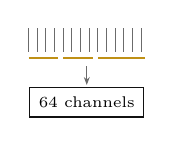
\begin{tikzpicture}[ic]
  \foreach \i in {0,...,13} \draw[mute] (\i*1.1,0) -- (\i*1.1,3);
  \foreach \a/\b in {0/3.8,4.4/8.2,8.8/14.8} \draw[ochre!90!black, line width=0.6pt] (\a,-0.8) -- (\b,-0.8);
  \draw[-{Stealth[length=1mm]}, mute] (7.4,-1.8) -- (7.4,-4.2);
  \node[draw=ink, minimum width=12mm, minimum height=3.5mm, font=\fontsize{5.6}{6}\selectfont] at (7.4,-6.4) {64 channels};
  \end{tikzpicture}}
\newcommand{\icaug}{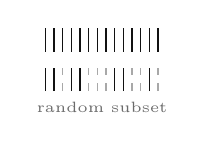
\begin{tikzpicture}[ic]
  \foreach \i in {0,...,13} \draw[ink] (\i*1.1,4) -- (\i*1.1,7);
  \foreach \i in {0,1,3,4,8,9,12} \draw[ink] (\i*1.1,-1) -- (\i*1.1,2);
  \foreach \i in {2,5,6,7,10,11,13} \draw[faint, dashed] (\i*1.1,-1) -- (\i*1.1,2);
  \node[font=\fontsize{5.4}{6}\selectfont, color=mute] at (7.2,-3) {random subset};
  \end{tikzpicture}}
\newcommand{\icseg}{
\begin{tikzpicture}[ic]
  \foreach \i in {0,...,4} \foreach \j in {0,...,4} \fill[natural!25] (\i*2.6,\j*2.6) rectangle ++(2.5,2.5);
  \foreach \i/\j in {0/4,1/4,0/3,3/1,4/1,4/0} \fill[natural!70] (\i*2.6,\j*2.6) rectangle ++(2.5,2.5);
  \foreach \i/\j in {2/3,3/3,3/4,2/4} \fill[faint!80] (\i*2.6,\j*2.6) rectangle ++(2.5,2.5);
  \end{tikzpicture}}
\newcommand{\icdec}{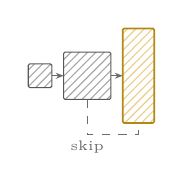
\begin{tikzpicture}[ic]
  \draw[ink!70, rounded corners=0.5pt, pattern=north east lines, pattern color=faint] (0,0) rectangle (3,3); \draw[ink!70, rounded corners=0.5pt, pattern=north east lines, pattern color=faint] (4.5,-1.5) rectangle (10.5,4.5);
  \draw[ochre!85!black, line width=0.6pt, rounded corners=0.5pt, pattern=north east lines, pattern color=ochre!50] (12,-4.5) rectangle (16,7.5);
  \draw[-{Stealth[length=1mm]}, mute] (3,1.5) -- (4.5,1.5); \draw[-{Stealth[length=1mm]}, mute] (10.5,1.5) -- (12,1.5);
  \draw[dashed, mute] (7.5,-1.5) -- (7.5,-6) -- (14,-6) -- (14,-4.5);
  \node[font=\fontsize{5}{6}\selectfont, color=mute] at (7.5,-7.5) {skip};
  \end{tikzpicture}}
\newcommand{\icheavy}{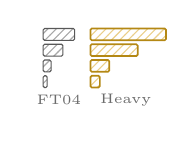
\begin{tikzpicture}[ic]
  \foreach \w/\y in {1/0,2/2,5/4,8/6} \draw[ink!70, rounded corners=0.5pt, pattern=north east lines, pattern color=faint] (0,\y) rectangle (\w*0.5,\y+1.5);
  \foreach \w/\y in {1/0,2/2,5/4,8/6} \draw[ochre!85!black, line width=0.6pt, rounded corners=0.5pt, pattern=north east lines, pattern color=ochre!50] (6,\y) rectangle (6+\w*1.2,\y+1.5);
  \node[font=\fontsize{5}{6}\selectfont, color=mute] at (2,-1.6) {FT04};
  \node[font=\fontsize{5}{6}\selectfont, color=mute] at (10.5,-1.6) {Heavy};
  \end{tikzpicture}}
\newcommand{\icrm}{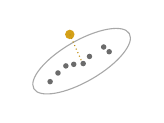
\begin{tikzpicture}[ic]
  \draw[faint, rotate=30] (0,0) ellipse (7 and 2.6);
  \foreach \p in {(-3,-1.5),(-1,-0.4),(1,0.6),(2.8,1.8),(0.2,-0.3),(-2,-0.6),(3.5,1.2),(-4,-2.6)} \fill[mute] \p circle (0.35);
  \fill[ochre] (-1.5,3.4) circle (0.6);
  \draw[ochre!90!black, densely dotted] (-1.5,3.4) -- (0,0);
  \end{tikzpicture}}
\newcommand{\ictried}{
\begin{tikzpicture}[ic]
  \node[draw=faint, dashed, minimum width=13mm, minimum height=9mm, text=mute, font=\fontsize{5.4}{6}\selectfont, align=center] {uncertainty\\head};
  \draw[manmade, line width=0.6pt] (4.5,-4.5) -- (7.5,-1.5) (4.5,-1.5) -- (7.5,-4.5);
  \end{tikzpicture}}
\newcommand{\icnamer}{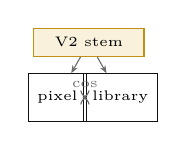
\begin{tikzpicture}[ic]
  \node[draw=ochre!90!black, fill=ochre!15, minimum width=14mm, minimum height=3mm, font=\fontsize{5}{6}\selectfont] (s) at (0,0) {V2 stem};
  \node[draw=ink, minimum width=5mm, minimum height=6mm, font=\fontsize{5}{6}\selectfont] (p) at (-4,-7) {pixel};
  \node[draw=ink, minimum width=5mm, minimum height=6mm, font=\fontsize{5}{6}\selectfont] (l) at (4,-7) {library};
  \draw[-{Stealth[length=1mm]}, mute] (s) -- (p); \draw[-{Stealth[length=1mm]}, mute] (s) -- (l);
  \draw[<->, mute] (p) -- node[above, font=\fontsize{5}{6}\selectfont]{cos} (l);
  \end{tikzpicture}}

\title{Allotrope v1.0}
\date{4 November 2026}

\begin{document}

%======================================================================
% 1 TITLE
%======================================================================
\begin{frame}[plain]
\begin{columns}[T,onlytextwidth]
\column{0.56\textwidth}
\vspace*{8mm}
{\fontsize{30}{32}\selectfont Allotrope v1.0\par}
\vspace{2mm}
{\fontsize{12.5}{15}\selectfont Hyperspectral anomaly detection\\ and material identification\par}
\vspace{3mm}
{\color{rule}\rule{0.9\linewidth}{0.4pt}}\par\vspace{2mm}
{\small Any sensor in, georeferenced answers out:\\
a boolean anomaly map, objects called \mm{} or \nat, and the closest material class.\par}
\vspace{5mm}
{\footnotesize AIGC Stage-III evaluation\\
Team Allotrope \textperiodcentered{} 4 November 2026, 09:00\par}
\vspace{6mm}
\begin{tabular}{@{}lll@{}}
\toprule
{\fontsize{16}{18}\selectfont 0.189} & {\fontsize{16}{18}\selectfont 449\,/\,909} & {\fontsize{16}{18}\selectfont +0.17} \\
\scriptsize pAUC, false alarms $\le$1\,\% & \scriptsize objects in the top 1\,\% & \scriptsize \mm{} recall over ACE\\
\scriptsize HyperSL: 0.095 & \scriptsize HyperSL: 369 & \scriptsize PRISMA, quarter-pixel targets\\
\bottomrule
\end{tabular}
%% src: 0.189 / 449 / 909 and HyperSL 0.0947 / 369: research/experiments/hypersl-anomaly-bench/README.md (cloud excl. rows)
%% src: +0.17: research/experiments/spectral-namer/N001b/README.md (level 1 passes by +0.20, +0.17, +0.14; PRISMA 0.94 vs ACE 0.77)
\column{0.42\textwidth}
\vspace*{4mm}
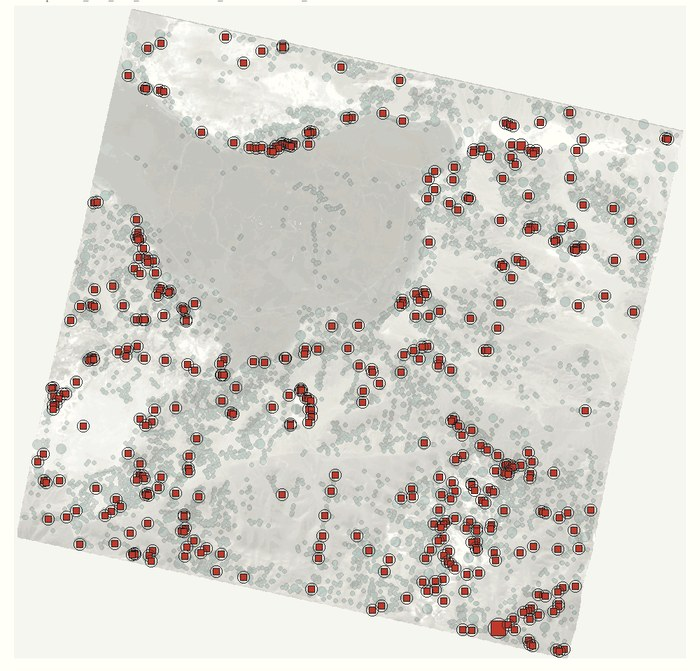
\includegraphics[width=\linewidth]{figures/story_prisma_k7.jpg}\par
\src{PRISMA, 14 Feb 2025: 405 man-made objects of 5,544 anomalies.}
%% src: docs/lld/spectral-namer-in-product.md (class-driven match screen: PRISMA 5,544 objects, 405 man-made)
\end{columns}
\end{frame}

%======================================================================
% 2 SCENE TO MATERIALS
%======================================================================
\begin{frame}{Scene to materials}
\vspace*{0.5mm}{\setlength{\tabcolsep}{0pt}
\begin{tabular}{@{}*{7}{>{\raggedright\arraybackslash}p{21.1mm}}@{}}
\sfr1&\sfr2&\sfr3&\sfr4&\sfr5&\sfr6&\sfr7\\[-0.5mm]
\scriptsize\textbf{1 Scene}&\scriptsize\textbf{2 Band filter}&\scriptsize\textbf{3 Segmentation}&\scriptsize\textbf{4 Score}&\scriptsize\textbf{5 Threshold}&\scriptsize\textbf{6 Namer}&\scriptsize\textbf{7 Selection}\\
\fontsize{6.4}{7.4}\selectfont 1237$\times$1202 px, 239 bands&
\fontsize{6.4}{7.4}\selectfont 186 of 239 bands usable; 30.3\,\% no-data&
\fontsize{6.4}{7.4}\selectfont thick cloud left out, 4.9\,\%&
\fontsize{6.4}{7.4}\selectfont Indradhanu V2 scores every pixel&
\fontsize{6.4}{7.4}\selectfont top 8\,\%: 118,950 pixels&
\fontsize{6.4}{7.4}\selectfont 5,544 objects&
\fontsize{6.4}{7.4}\selectfont\leavevmode{\color{manmade}405 man-made}
\end{tabular}\par}
%% src: captions of the story GIF key frames 1-7 for PRISMA PRS_L2D_STD_20250214052558 (scratchpad final/story/..._prisma_default/key1-7.png; docs/lld/story-gif.md)
\take{One PRISMA scene, 1.5 million pixels, narrowed in seven recorded steps to the objects an analyst asks for.}
\vspace{2.5mm}
\begin{columns}[T,onlytextwidth]
\column{0.50\textwidth}
\kicker{the same chain on three sensors}\par\vspace{0.6mm}
\fitw{\scriptsize\begin{tabular}{@{}lrrr@{}}
\toprule
& Tanager & PRISMA & AVIRIS-NG\\
\midrule
anomaly objects & 1,103 & 5,544 & 2,375\\
\mm{} at $P(\mathrm M)>0.5$ & 272 & 405 & 1,290\\
\mm{} at 0.25 (very sensitive) & 585 & 2,263 & 1,716\\
oil/fuel + plastic & 247 & 141 & 936\\
\bottomrule
\end{tabular}}\par
%% src: docs/lld/spectral-namer-in-product.md section 6, class-driven match screen table
\column{0.46\textwidth}
\kicker{what the evaluators receive per scene}\par\vspace{0.6mm}
{\fontsize{7}{8.6}\selectfont
\textbf{Map}: boolean anomaly mask, GeoTIFF on the scene's UTM grid\par
\textbf{Vectors}: pixel and object shapefiles with call, class and SAM match\par
\textbf{Table}: one row per object, with latitude and longitude\par
\textbf{Reflectance}: L2 surface reflectance from L1, GeoTIFF and BSQ\par
\textbf{No heatmap} in any submission pack\par}
%% src: docs/lld/spectral-namer-in-product.md (class-driven pack); C:/wt/atm-docker/isofit-atm-docker/README.md (L2_SR product)
\end{columns}
\end{frame}

%======================================================================
% 3 PIPELINE
%======================================================================
\begin{frame}{Pipeline}
\centering
\resizebox{\textwidth}{!}{%
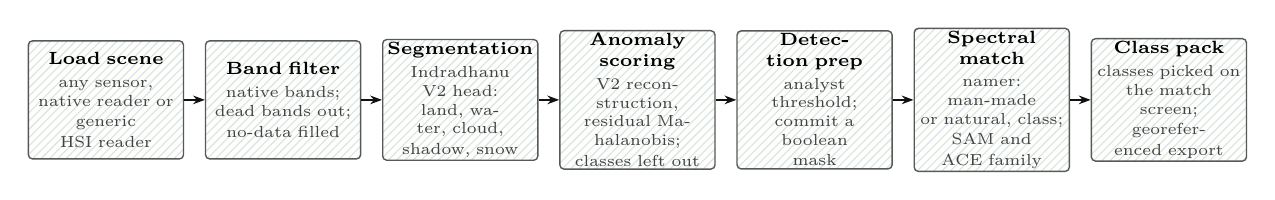
\begin{tikzpicture}[x=1mm,y=1mm]
\foreach \i/\t/\b in {
 {0/Load scene/any sensor,\\native reader or\\generic HSI reader},
 {1/Band filter/native bands;\\dead bands out;\\no-data filled},
 {2/Segmentation/Indradhanu V2 head:\\land, water, cloud,\\shadow, snow},
 {3/Anomaly scoring/V2 reconstruction,\\residual Mahalanobis;\\classes left out},
 {4/Detection prep/analyst threshold;\\commit a boolean\\mask},
 {5/Spectral match/namer: man-made\\or natural, class;\\SAM and ACE family},
 {6/Class pack/classes picked on\\the match screen;\\georeferenced export}}{
  \node[stg, pattern color=pB!90, minimum width=19mm, minimum height=15mm, text width=19mm] (n\i) at (\i*22.5, 0)
    {\textbf{\upshape\t}\\[0.5mm]{\upshape\color{ink!80}\fontsize{5.8}{6.8}\selectfont \b}};}
\foreach \i [evaluate=\i as \j using int(\i+1)] in {0,...,5} \draw[df] (n\i.east) -- (n\j.west);
\end{tikzpicture}}
%% src: docs/proposals/class-driven-flow.md ("The flow", steps 1-7)
\take{Seven actions in one dependency graph; each step writes what the next reads, and the export restores the scene's real map grid.}
\vspace{2mm}
\begin{columns}[T,onlytextwidth]
\column{0.31\textwidth}
\kicker{time per PRISMA scene, CPU, 16 threads}\par\vspace{0.4mm}
\fitw{\scriptsize\begin{tabular}{@{}lr@{}}
\toprule
V2 reconstruction, two passes & 402 s\\
V2 segmentation & 47 s\\
residual Mahalanobis & 4 s\\
\textbf{V2 total} (FT04: 274 s) & \textbf{454 s}\\
namer, PRISMA / Tanager & 9.2 / 7.6 s\\
class-pack export & 2.1--2.6 s\\
\bottomrule
\end{tabular}}\par
%% src: FTH3-heavy-joint-more2/README.md (16 threads: 454 = predict 402, segment 47, score 4; FT04 274); docs/lld/spectral-namer-in-product.md (9.2/7.6 s; export 2.1-2.6 s)
\column{0.33\textwidth}
\kicker{how it runs}\par\vspace{0.4mm}
\begin{itemize}\setlength{\itemsep}{0.3mm}\scriptsize
\item The job queue is a Postgres table with row locking and heartbeats; no message broker.
\item A web API and one worker; the browser polls. One origin behind nginx.
\item Science code never touches the database.
\end{itemize}
%% src: CLAUDE.md (Key facts; Layering rule)
\column{0.32\textwidth}
\kicker{sensors end to end}\par\vspace{0.4mm}
\fitw{\scriptsize\begin{tabular}{@{}ll@{}}
\toprule
hyperspectral & PRISMA, EnMAP, AVIRIS-NG, Tanager\\
any HSI file & GeoTIFF, ENVI, HDF5, NetCDF\\
& (GHOSt is the first user)\\
thermal & Landsat-9, HotSat-1 (Chakshu)\\
\bottomrule
\end{tabular}}\par
%% src: CLAUDE.md (sensors); docs/lld/tanager.md; docs/lld/generic-hsi.md
\end{columns}
\end{frame}

%======================================================================
% 4 ARCHITECTURE EVOLUTION
%======================================================================
\begin{frame}{Architecture evolution}
\centering
% Architecture evolution of Indradhanu: one mini schematic per generation; new parts in ochre.
% Sources: docs/04-models.md, docs/lld/spectral-stem.md, docs/lld/evaluation.md, research/experiments/indradhanu-se-pretrain/F002-heavy/README.md,
% research/experiments/indradhanu-finetune/FTH3-heavy-joint-more2/README.md, final design/ROADMAP.md (OB-14), git log dates.
\newcommand{\gen}[8]{% x, input, stem style, stem, encoder style, encoder, decoder style, decoder
  \node[lab, color=mute] at (#1,0) {#2};
  \node[#3, minimum width=17mm, minimum height=3.6mm] at (#1,-4.5) {#4};
  \node[#5, minimum height=4.2mm] at (#1,-9.6) {#6};
  \node[#7, minimum width=17mm, minimum height=3.6mm] at (#1,-14.7) {#8};
  \draw[ar] (#1,-1.6) -- (#1,-2.6); \draw[ar] (#1,-6.4) -- (#1,-7.4); \draw[ar] (#1,-11.8) -- (#1,-12.8); \draw[ar] (#1,-16.6) -- (#1,-17.7);}
\adjustbox{max width=\textwidth, max totalheight=0.42\textheight}{%
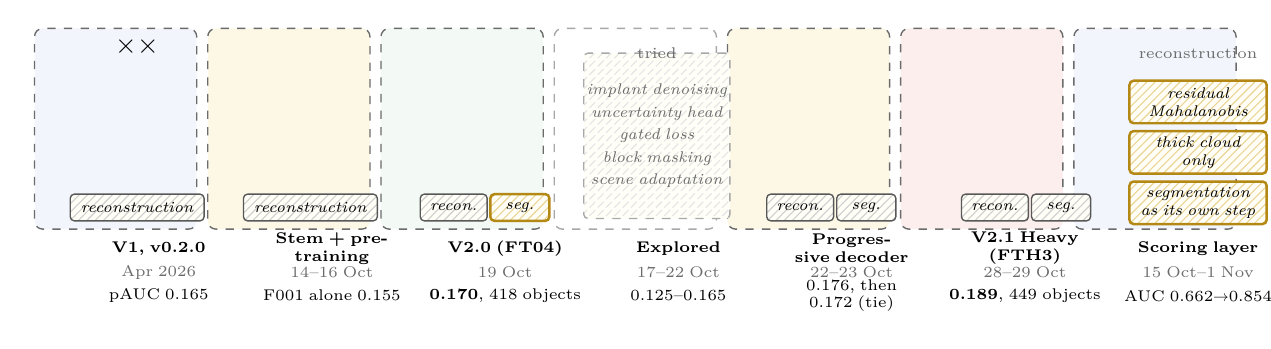
\begin{tikzpicture}[x=1mm,y=1mm,
  mb/.style={stg, pattern color=faint!55, inner sep=0.6pt, font=\itshape\fontsize{5.6}{6.4}\selectfont},
  nw/.style={stgn, inner sep=0.6pt, font=\itshape\fontsize{5.6}{6.4}\selectfont},
  ex/.style={stgx, dashed, inner sep=0.8pt, font=\itshape\fontsize{5.6}{6.4}\selectfont},
  lab/.style={font=\fontsize{5.6}{6.4}\selectfont, align=center, text width=20mm},
  ar/.style={-{Stealth[length=1mm,width=0.8mm]}, line width=0.35pt, draw=mute}]
\gen{0}{165-band grid}{mb}{1$\times$1 compressor}{mb, minimum width=10mm}{encoder}{mb}{SegFormer decoder}
\node[mb, minimum width=17mm, minimum height=3.4mm] at (0,-19.6) {reconstruction};
\gen{22}{\textcolor{ochre!80!black}{\textbf{any band list}}}{nw}{wavelength stem}{mb, minimum width=10mm}{encoder}{mb}{SegFormer decoder}
\node[mb, minimum width=17mm, minimum height=3.4mm] at (22,-19.6) {reconstruction};
\gen{44}{native bands}{mb}{wavelength stem}{mb, minimum width=10mm}{encoder}{mb}{SegFormer decoder}
\node[mb, minimum width=8.5mm, minimum height=3.4mm] at (40.2,-19.6) {recon.};
\node[nw, minimum width=7.5mm, minimum height=3.4mm] at (48.6,-19.6) {seg.};
\node[ex, text width=18mm, minimum height=21mm] at (66,-10.5) {implant denoising\\[0.6mm] uncertainty head\\[0.6mm] gated loss\\[0.6mm] block masking\\[0.6mm] scene adaptation};
\node[lab, color=mute] at (66,0) {tried};
\gen{88}{native bands}{mb}{wavelength stem}{mb, minimum width=10mm}{encoder}{nw}{progressive decoder}
\node[mb, minimum width=8.5mm, minimum height=3.4mm] at (84.2,-19.6) {recon.};
\node[mb, minimum width=7.5mm, minimum height=3.4mm] at (92.6,-19.6) {seg.};
\gen{110}{native bands}{mb}{wavelength stem, 64}{nw, minimum width=18mm}{encoder, 3$\times$ wide}{mb}{progressive decoder}
\node[mb, minimum width=8.5mm, minimum height=3.4mm] at (106.2,-19.6) {recon.};
\node[mb, minimum width=7.5mm, minimum height=3.4mm] at (114.6,-19.6) {seg.};
\node[lab, color=mute] at (132,0) {reconstruction};
\node[nw, text width=17mm, minimum height=5.4mm] at (132,-6.2) {residual\\Mahalanobis};
\node[nw, text width=17mm, minimum height=5.4mm] at (132,-12.6) {thick cloud\\only};
\node[nw, text width=17mm, minimum height=5.4mm] at (132,-19) {segmentation\\as its own step};
\foreach \x/\n/\d/\r in {
  {0/V1, v0.2.0/Apr 2026/pAUC 0.165},
  {22/Stem + pretraining/14--16 Oct/F001 alone 0.155},
  {44/V2.0 (FT04)/19 Oct/\textbf{0.170}, 418 objects},
  {66/Explored/17--22 Oct/0.125--0.165},
  {88/Progressive decoder/22--23 Oct/0.176, then 0.172 (tie)},
  {110/V2.1 Heavy (FTH3)/28--29 Oct/\textbf{0.189}, 449 objects},
  {132/Scoring layer/15 Oct--1 Nov/AUC 0.662$\to$0.854}}
  {\node[lab] at (\x,-24.8) {\textbf{\n}};
   \node[lab, color=mute] at (\x,-27.8) {\d};
   \node[lab] at (\x,-30.8) {\r};}
\begin{scope}[on background layer]
\foreach \x/\f in {0/pB,22/pY,44/pG,88/pY,110/pR,132/pB} \node[grp, fill=\f!28, minimum width=20.6mm, minimum height=25.5mm, inner sep=0] at (\x,-9.6) {};
\node[grp, draw=faint, minimum width=20.6mm, minimum height=25.5mm, inner sep=0] at (66,-9.6) {};
\end{scope}
\end{tikzpicture}}

\vspace{1mm}
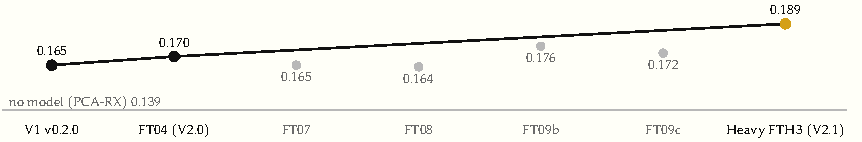
\includegraphics[width=\textwidth]{figures/chart_generations.pdf}
%% src: pAUC (cloud excluded): v0.2.0 0.165 and FT04 0.170 (final design/ROADMAP.md OB-14); FT07 0.165, FT08 0.164, FT09b 0.176, FT09c 0.172 (docs/lld/evaluation.md);
%% src:   FTH3 0.189 (FTH3 README); F001 pretrained 0.155 (F002-heavy README); no model PCA-RX 0.139 (hypersl-anomaly-bench README); FT06 0.125/0.163, scene adaptation ~0.160 (evaluation.md); 418 = 46.0% of 909 (FTH3 eval_report.md)
%% src: dates: git log (d2f8c3c 2026-04-10; 392e106/64f0106 2026-10-14..16; 20afa70 2026-10-19; 8c14fe6/43ddd53 2026-10-22; b410671 2026-10-23; a0b6930/c4b3a63 2026-10-28/29; 4b7da29 2026-10-15; 53ac8d7 2026-11-01)
\take{Shipped generations in ink, experiments that did not beat the shipped model in grey; each column adds the part outlined in ochre.}
\end{frame}

%======================================================================
% 5 V1 AND V2
%======================================================================
\begin{frame}{Indradhanu V1 and V2}
\centering
% Indradhanu V1 (v0.2.0) against V2 (Heavy, v2.1.0), in the grouped/hatched style; V2's new parts outlined in ochre.
% Sources: docs/04-models.md (V1: 165-band grid, 1x1 compressor to 24-32 channels, SegFormer MAE, pixel-shuffle decoder, 5.5 M;
% V2: wavelength stem, [96,192,480,768], heads [3,6,10,12], progressive decoder 512 -> 256/128, 35.3 M);
% docs/lld/spectral-stem.md (40 nm bins, per-band skip, thick-cloud rule); research/textbook/chapters/41-heavy.tex (33,884,194 + 1,431,120).
\adjustbox{max width=\textwidth, max totalheight=0.74\textheight}{%
\begin{tikzpicture}[x=1mm,y=1mm]
% ---------------- V1 ----------------
\node[grp, fill=pB!35, minimum width=176mm, minimum height=24mm, anchor=north west] (G1) at (0,0) {};
\node[glab] at (G1.north west) {Indradhanu V1 (v0.2.0) \textperiodcentered{} 5.5\,M parameters \textperiodcentered{} one fixed grid};
\node[inner sep=0, anchor=west] (i1) at (4,-13) {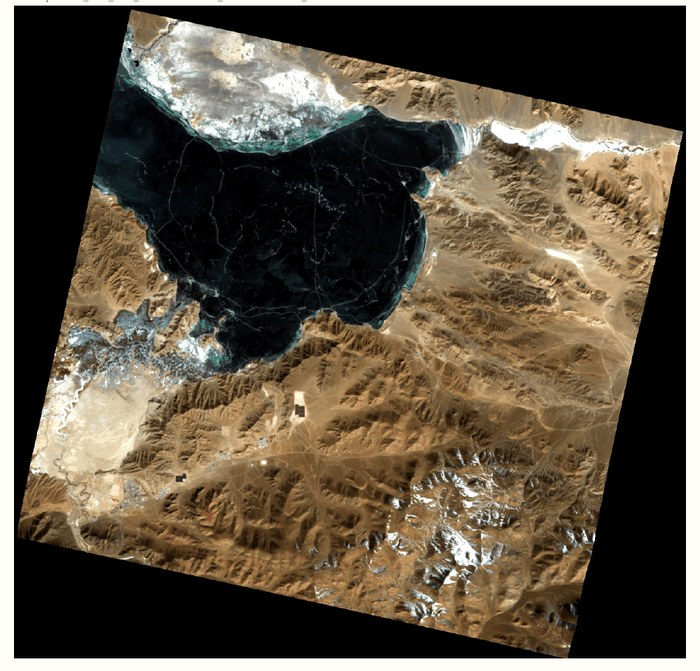
\includegraphics[width=12mm]{figures/story_prisma_k1.jpg}};
\node[tsh, below=0.3mm of i1] {165-band grid};
\node[stg, minimum width=15mm, minimum height=10mm] (c1) at (31,-13) {1$\times$1\\compressor};
\node[tsh, above=0.4mm of c1] {165 $\to$ 24--32 ch};
\node[grp, fill=pG!30, minimum width=58mm, minimum height=17mm] (E1) at (75,-13.5) {};
\node[glab] at (E1.north west) {Encoder};
\foreach \i/\x in {1/53,2/67,3/81,4/95} {
  \node[stg, minimum width=11mm, minimum height=9mm] (s1\i) at (\x,-14.5) {};
  \node[font=\itshape\fontsize{6}{7}\selectfont] at (\x,-12.2) {stage \i};
  \node[cell, fill=pG] at (\x-1.4,-16.4) {}; \node[cell, fill=pG] at (\x+1.4,-16.4) {};}
\foreach \i [evaluate=\i as \j using int(\i+1)] in {1,2,3} \draw[df] (s1\i) -- (s1\j);
\node[grp, fill=pY!35, minimum width=20mm, minimum height=17mm] (D1) at (120,-13.5) {};
\node[glab] at (D1.north west) {Decoder};
\node[stg, minimum width=14mm, minimum height=9mm] (d1) at (120,-14.5) {SegFormer\\pixel shuffle};
\node[font=\fontsize{7}{8}\selectfont] (o1) at (143,-13) {$\hat{\mathbf x}$};
\node[loss] (l1) at (156,-8) {L1 + SAM};
\node[loss] (r1) at (156,-18) {combined score};
\draw[df] (i1) -- (c1); \draw[df] (c1) -- (s11); \draw[df] (s14) -- (d1); \draw[df] (d1) -- (o1);
\draw[tf] (o1) -- (l1); \draw[df] (o1) -- (r1);
% ---------------- V2 ----------------
\node[grp, fill=pR!30, minimum width=176mm, minimum height=40mm, anchor=north west] (G2) at (0,-28) {};
\node[glab] at (G2.north west) {Indradhanu V2 (v2.1.0, Heavy) \textperiodcentered{} 33.9\,M + 1.43\,M head = 35.3\,M parameters \textperiodcentered{} any sensor};
\node[inner sep=0, anchor=west] (i2) at (4,-46) {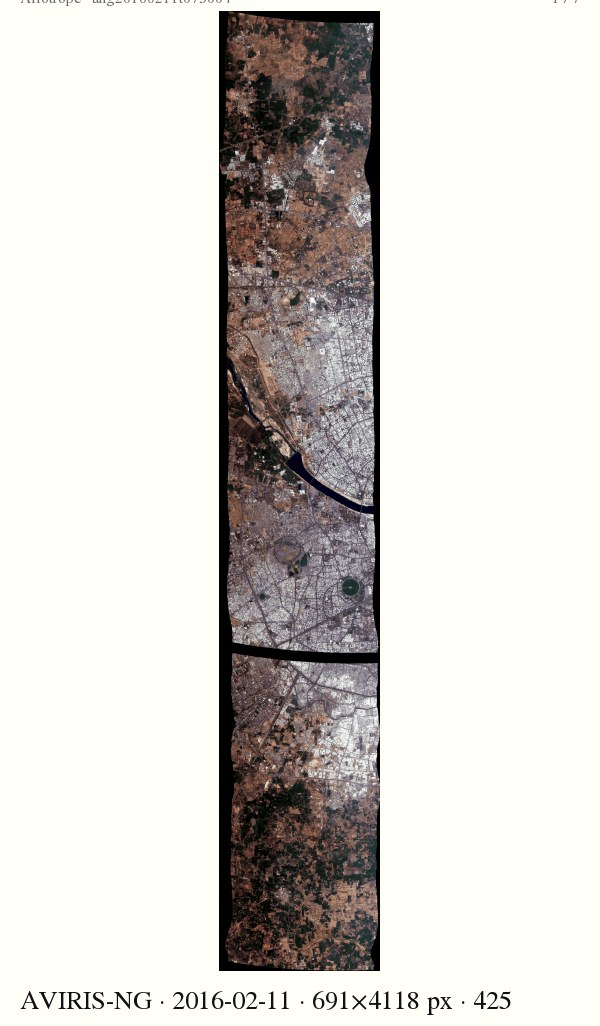
\includegraphics[width=12mm]{figures/story_aviris_k1.jpg}};
\draw[ochre!85!black, line width=0.6pt] plot[smooth] coordinates {(4,-60) (6,-58.2) (8,-57.5) (9.5,-59.5) (11,-56.8) (13,-57.3) (16,-58.6)};
\node[tsh, text=ochre!80!black] at (10,-62.5) {any bands, native};
% stem
\node[grp, fill=pY!30, draw=ochre!85!black, solid, minimum width=30mm, minimum height=26mm] (S2) at (37,-47) {};
\node[glab] at (S2.north west) {Spectral stem};
\foreach \k in {0,...,6} \node[cell, fill=pY] at (26.5+\k*2.9,-42.4) {};
\node[tsh] at (35.2,-39.8) {40\,nm wavelength bins};
\foreach \k in {0,...,3} \node[cell, circle, fill=pB] at (30.8+\k*2.9,-47.5) {};
\node[tsh] at (35.2,-51) {attention, 4 heads};
\node[stgn, minimum width=13mm, minimum height=4.5mm] (z2) at (35.2,-56.4) {64 ch};
\draw[df] (35.2,-43.6) -- (35.2,-45.8); \draw[df] (35.2,-49.2) -- (z2);
% encoder
\node[grp, fill=pG!30, draw=ochre!85!black, solid, minimum width=62mm, minimum height=26mm] (E2) at (90,-47) {};
\node[glab] at (E2.north west) {Encoder, 3$\times$ wider};
\foreach \i/\x/\w/\c/\h in {1/68/8/96/3,2/80/10/192/6,3/94/12.5/480/10,4/110/15/768/12} {
  \node[stgn, minimum width=\w mm, minimum height=11mm] (s2\i) at (\x,-48) {};
  \node[font=\itshape\fontsize{6}{7}\selectfont] at (\x,-45.2) {stage \i};
  \node[cell, fill=pG] at (\x-1.4,-49) {}; \node[cell, fill=pG] at (\x+1.4,-49) {};
  \node[font=\itshape\fontsize{5.2}{6}\selectfont] at (\x,-51.6) {\c, \h\ h};}
\foreach \i [evaluate=\i as \j using int(\i+1)] in {1,2,3} \draw[df] (s2\i) -- (s2\j);
% decoder
\node[grp, fill=pY!30, draw=ochre!85!black, solid, minimum width=24mm, minimum height=26mm] (D2) at (138,-47) {};
\node[glab] at (D2.north west) {Decoder};
\node[stgn, minimum width=18mm, minimum height=5mm] (u1) at (138,-43.5) {fuse 512 $\to$ 256};
\node[stgn, minimum width=18mm, minimum height=5mm] (u2) at (138,-52.5) {up 256 $\to$ 128};
\draw[df] (u1) -- (u2);
% heads
\node[font=\fontsize{7}{8}\selectfont] (o2) at (158,-40) {$\hat{\mathbf x}$};
\node[loss] (l2) at (173,-36) {L1 + SAM};
\node[loss] (r2) at (173,-44.5) {Mahalanobis};
\node[stgn, minimum width=13mm, minimum height=7mm] (h2) at (164,-58) {seg head};
\node[tsh] at (164,-63.6) {land water cloud shadow snow};
\node[loss] (b2) at (176,-52) {BCE+Dice};
% flows
\draw[df] (i2) -- (S2.west |- i2); \draw[df] (z2.east) -- (s21.west |- z2.east) ;
\draw[df] (s24) -- (u1.west |- s24);
\draw[df] (u2.east) -| (o2.south);
\draw[tf] (o2) -- (l2); \draw[df] (o2) -- (r2);
\draw[tf, draw=ochre!85!black] (s24.north) -- (110,-31.5) -| (h2.north);
\draw[tf] (h2) -- (b2);
\draw[tf] (z2.south) -- ++(0,-6.5) -| node[pos=0.3, tsh, above]{skip at full resolution, hidden pixels zeroed} (u2.south);
% ---------------- legend ----------------
\begin{scope}[shift={(4,-75)}]
\node[stg, minimum width=7mm, minimum height=3.5mm] at (3,0) {}; \node[tsh, anchor=west, text=ink] at (7.5,0) {stage block};
\node[cell, fill=pG] at (30,0) {}; \node[cell, fill=pY] at (32.5,0) {}; \node[cell, circle, fill=pB] at (35,0) {}; \node[tsh, anchor=west, text=ink] at (37,0) {cells: transformer blocks, wavelength bins, attention heads};
\node[loss] at (101,0) {loss}; \node[tsh, anchor=west, text=ink] at (105,0) {loss / score};
\draw[df] (124,0) -- (131,0); \node[tsh, anchor=west, text=ink] at (132,0) {data flow};
\draw[tf] (147,0) -- (154,0); \node[tsh, anchor=west, text=ink] at (155,0) {training-only / optional};
\draw[ochre!85!black, line width=0.9pt, rounded corners=1pt] (-1,-4.5) rectangle (6,-2.6); \node[tsh, anchor=west, text=ink] at (7.5,-3.6) {new in V2};
\end{scope}
\end{tikzpicture}}

\take{V1 v0.2.0 0.165 $\to$ V2 FT04 0.170 $\to$ V2 Heavy 0.189 pAUC on the labelled PRISMA bench, cloud excluded; 418 $\to$ 449 of 909 objects in the top 1\,\%.}
%% src: 0.165/0.170 final design/ROADMAP.md OB-14; 0.189/449 FTH3 README + hypersl-anomaly-bench README; 418 = 46.0% (eval_report.md)
\end{frame}

%======================================================================
% 6 INDRADHANU V2 IN DETAIL
%======================================================================
\begin{frame}{Indradhanu V2}
\centering
% Indradhanu V2 (Heavy, v2.1.0) block diagram; shapes recorded by forward hooks (research/textbook/chapters/41-heavy.tex)
\adjustbox{max width=\textwidth, max totalheight=0.52\textheight}{%
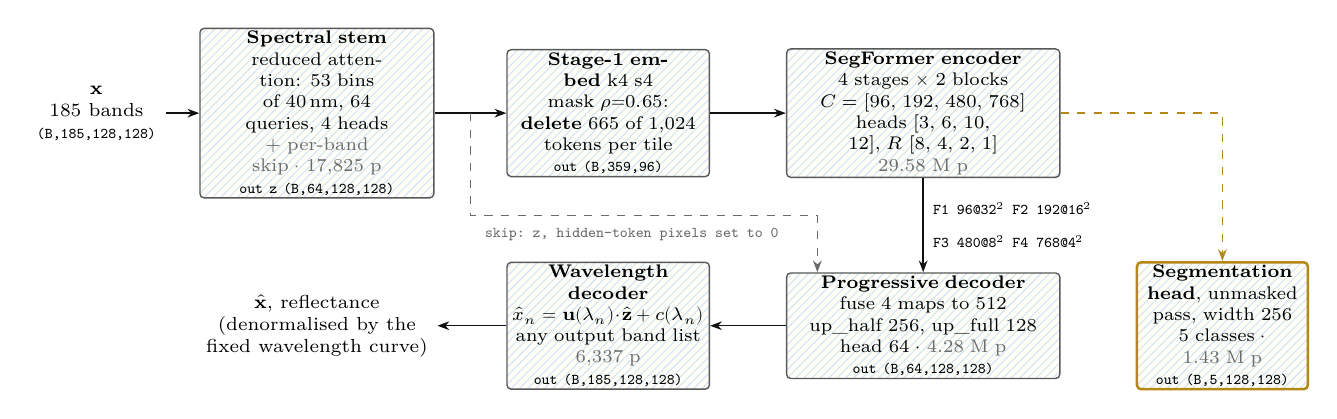
\begin{tikzpicture}[x=1mm,y=1mm]
\tikzset{blk/.style={stg, pattern color=pB!85, minimum height=12mm, font=\fontsize{6.6}{7.7}\selectfont}}
\node[font=\fontsize{6.8}{8}\selectfont, align=center] (x) at (-4,0) {$\mathbf{x}$\\185 bands\\\shp{(B,185,128,128)}};
\node[blk, text width=29mm] (A) at (24,0) {\textbf{Spectral stem}\\reduced attention: 53 bins\\of 40\,nm, 64 queries, 4 heads\\{\color{mute}+ per-band skip $\cdot$ 17,825 p}\\\shp{out z (B,64,128,128)}};
\node[blk, text width=25mm] (B) at (61,0) {\textbf{Stage-1 embed} k4 s4\\mask $\rho{=}0.65$:\\\textbf{delete} 665 of 1,024\\tokens per tile\\\shp{out (B,359,96)}};
\node[blk, text width=34mm] (C) at (101,0) {\textbf{SegFormer encoder}\\4 stages $\times$ 2 blocks\\$C$ = [96, 192, 480, 768]\\heads [3, 6, 10, 12], $R$ [8, 4, 2, 1]\\{\color{mute}29.58 M p}};
\node[blk, text width=34mm] (D) at (101,-27) {\textbf{Progressive decoder}\\fuse 4 maps to 512\\up\_half 256, up\_full 128\\head 64 $\cdot$ {\color{mute}4.28 M p}\\\shp{out (B,64,128,128)}};
\node[blk, text width=25mm] (E) at (61,-27) {\textbf{Wavelength decoder}\\$\hat x_n=\mathbf{u}(\lambda_n)\!\cdot\!\hat{\mathbf z}+c(\lambda_n)$\\any output band list\\{\color{mute}6,337 p}\\\shp{out (B,185,128,128)}};
\node[font=\fontsize{6.8}{8}\selectfont, align=center] (y) at (24,-27) {$\hat{\mathbf{x}}$, reflectance\\(denormalised by the\\fixed wavelength curve)};
\node[blk, text width=21mm, draw=ochre!85!black, line width=0.9pt] (F) at (139,-27) {\textbf{Segmentation}\\\textbf{head}, unmasked\\pass, width 256\\5 classes $\cdot$ {\color{mute}1.43 M p}\\\shp{out (B,5,128,128)}};
\draw[df] (x) -- (A); \draw[df] (A) -- (B); \draw[df] (B) -- (C);
\draw[df] (C) -- node[right, align=left]{\shp{F1 96@32$^2$ F2 192@16$^2$}\\\shp{F3 480@8$^2$ F4 768@4$^2$}} (D);
\draw[df] (D) -- (E); \draw[df] (E) -- (y);
\draw[tf, draw=ochre!85!black] (C.east) -| (F.north);
\draw[tf] ($(A.east)!0.5!(B.west)$) -- ++(0,-13) -| ($(D.north west)+(4,0)$);
\node[color=mute, anchor=north] at (64,-13.4) {\shp{skip: z, hidden-token pixels set to 0}};
\end{tikzpicture}}

%% src: shapes and parameter counts: research/textbook/chapters/41-heavy.tex (forward-hook trace; stem 17,825, encoder 29,580,288, decoder 4,279,616, output 6,337, segmentation head 1,431,120)
\vspace{0.5mm}
\begin{columns}[T,onlytextwidth]
\column{0.53\textwidth}
\kicker{objective, on hidden pixels $M$ only}\par
\vspace{-1.5mm}
{\footnotesize
\[
\mathcal L=\underbrace{\tfrac{1}{C|M|}\!\sum_{p\in M}\sum_{c}|\hat x_{c,p}-x_{c,p}|}_{L_1}
+\lambda(t)\,\underbrace{\tfrac{1}{|M|}\!\sum_{p\in M}\angle(\mathbf x_p,\hat{\mathbf x}_p)}_{L_{\mathrm{SAM}}}
+\,0.1\,\mathcal L_{\mathrm{seg}}
\]\par}
\vspace{-1.5mm}
{\fontsize{6.4}{7.6}\selectfont $\lambda(t)=0.5\min(1,t/10)$; $\mathcal L_{\mathrm{seg}}$ = BCE + Dice. A pixel is always scored from the pass in which it was hidden.\par}
%% src: research/textbook/chapters/23-losses.tex (L1 + lambda(t) SAM, ramp); 27-finetune.tex (seg_weight 0.1 x masked BCE + Dice); docs/04-models.md (two-pass complementary masking)
\column{0.44\textwidth}
\kicker{as trained}\par\vspace{0.3mm}
\fitw{\fontsize{6.4}{7.6}\selectfont\begin{tabular}{@{}lll@{}}
\toprule
& pretraining (F002) & fine-tuning (FTH3)\\
\midrule
data & SpectralEarth & EnMAP, PRISMA, AVIRIS-NG\\
epochs & 80 & 18 + 6\\
learning rate, cosine & $3\!\times\!10^{-4}$ & $3\!\times\!10^{-5}$\\
batch & 32, bf16, 1 H100 & 16 $\times$ 2, bf16\\
mask ratio & 0.65 & 0.65\\
validation SAM & 3.89$^\circ$ & PRISMA 4.48$^\circ$\\
\bottomrule
\end{tabular}}\par
%% src: F002-heavy/config.json + README.md (80 epochs, lr 3e-4, batch 32, mask_ratio 0.65, val SAM 3.89); FTH3 config.json (lr 3e-5, 16x2, 6 epochs) + README.md (FTH2 18 joint epochs + 6; ep5 PRISMA SAM 4.48)
\end{columns}
\end{frame}

%======================================================================
% 7-8 COMPONENTS
%======================================================================
\begin{frame}{Components}
\vspace{1mm}
\card{\icstem}{Wavelength-aware spectral stem}{Attention over 40\,nm wavelength bins (53 bins, 64 queries, 4 heads) plus a per-band skip path into 64 channels. Takes any band list; 17,825 parameters.}{About 6$\times$ faster than per-band attention at equal detail; reads PRISMA's 185 native bands without resampling.}{\shipped}\hfill
\card{\icaug}{Band-list augmentation}{80\,\% of training batches read a random band subset (50--95\,\% thinning, 1--3 gaps of 20--150\,nm, or a 6--15\,nm grid; never under 40 bands); stated wavelengths jittered $\pm$3\,nm.}{Fixes the failure it was built for: before it, native PRISMA Set-1 scored ROC-AUC 0.205 against 0.725 when resampled.}{\shipped}\par
\vspace{2mm}
\card{\icseg}{Segmentation head}{An unmasked pass through the same encoder into a width-256 head: land, water, cloud, thin cloud, shadow, snow. 1.43\,M parameters.}{IoU water 0.825, cloud 0.749. Excluding thick cloud only lifts pAUC 0.175 $\to$ 0.189.}{\shipped}\hfill
\card{\icdec}{Progressive decoder}{Fuse the four encoder maps to 512, then up-sample 256 $\to$ 128 with a full-resolution skip from the stem, hidden pixels zeroed.}{Alone (FT09b): +0.0060 [+0.0002, +0.0118] pAUC, then a tie five epochs later. Kept in Heavy, pretrained from the start.}{\shipped}
%% src: stem: docs/lld/spectral-stem.md (53 bins, 40 nm, reduced attention ~6x faster), research/textbook/chapters/41-heavy.tex (64 queries, 4 heads, 17,825; 185 kept)
%% src: augmentation: FTH3/F002 config band_augment_prob 0.8, band_jitter_nm 3; docs/lld/spectral-stem.md (thinning 50-95%, 1-3 gaps 20-150 nm, 6-15 nm grid, >=40 bands; E004 set1 ROC-AUC 0.205 native vs 0.725 resampled)
%% src: seg head: 41-heavy.tex (width 256, 1,431,120); FTH3 finetune_metrics.csv ep5 (0.8246, 0.7487); eval_report.md (RM 0.175 -> thick excl 0.189)
%% src: progressive decoder: 41-heavy.tex (fuse 512, up_half 256, up_full 128, skip zeroed); docs/lld/evaluation.md (FT09b +0.0060 [+0.0002, +0.0118]; FT09c tie)
\end{frame}

\begin{frame}{Components, continued}
\vspace{1mm}
\card{\icheavy}{Heavy scaling}{Encoder widths $\times$3, [96, 192, 480, 768], heads [3, 6, 10, 12]; spectral width 64; 33.9\,M parameters. 80 epochs on one H100.}{Pretrained alone 0.166 vs 0.155; fine-tuned 0.189 vs FT04's 0.170, +0.0196 [+0.0072, +0.0316].}{\shipped}\hfill
\card{\icrm}{Residual Mahalanobis score}{Whiten the reconstruction residual in its top 30 directions; measure each pixel against the mean of a ring (21/61 px) of neighbours.}{Mean ROC-AUC 0.662 $\to$ 0.854 on the same model; 3--4\,s per scene.}{\shipped}\par
\vspace{2mm}
\card{\ictried}{Uncertainty head, gated training}{A per-pixel scale head (FT06); a gated loss (FT07) and block masking (FT08); implant denoising (FT05); per-scene adaptation.}{Uncertainty 0.125 / 0.163, gated loss 0.165, block masking 0.164, adaptation $\approx$0.160, all against 0.170. None shipped.}{\tried}\hfill
\card{\icnamer}{Spectral namer}{Two towers on V2's stem and normalisation (17,825 of 347,685 parameters) match a pixel against library spectra.}{Man-made recall at ACE's false-alarm rate +0.14 to +0.20 over ACE at quarter-pixel fill.}{\shipped}
%% src: Heavy: F002-heavy README/config ([96,192,480,768], [3,6,10,12], 64, 33.9 M, 80 epochs, 0.166 vs 0.155); FTH3 bootstrap.txt (+0.0196 [+0.0072, +0.0316])
%% src: RM: docs/lld/residual-mahalanobis.md (d=30, 21/61, 3-4 s); dual-window-mahalanobis/README.md (0.662 -> 0.854)
%% src: tried: docs/lld/evaluation.md (FT06 0.125 / 0.163; FT07 0.165; FT08 0.164; scene adaptation ~0.160 vs 0.170)
%% src: namer: research/textbook/chapters/42-namer.tex (347,685; stem 17,825); N001b README (+0.20 / +0.17 / +0.14)
\end{frame}

%======================================================================
% 9 ANOMALY SCORE
%======================================================================
\begin{frame}{Anomaly score}
\begin{columns}[T,onlytextwidth]
\column{0.48\textwidth}
\kicker{per pixel $p$}\par
\vspace{-1mm}
{\small
\begin{align*}
\mathbf r_p&=\mathbf x_p-\hat{\mathbf x}_p\in\mathbb R^{C}\\
\mathbf z_p&=\boldsymbol\Lambda_d^{-1/2}\mathbf U_d^{\top}(\mathbf r_p-\boldsymbol\mu_r),\quad d=30\\
s(p)&=\Big\|\mathbf z_p-\tfrac{1}{|\mathcal R_p|}\textstyle\sum_{q\in\mathcal R_p}\mathbf z_q\Big\|^2
\end{align*}\par}
\vspace{-1mm}
\begin{itemize}\setlength{\itemsep}{0.4mm}\scriptsize
\item $\mathbf U_d,\boldsymbol\Lambda_d$: top 30 eigenpairs of the residual covariance over up to 200,000 valid pixels. Stabilised by truncation; 465 covariance entries instead of 17,205 for 185 bands.
\item $\mathcal R_p$: the 3,280-pixel ring between a 21$\times$21 guard and a 61$\times$61 window, summed with integral images in four look-ups.
\item Plain RX over all bands was dropped: near-singular covariance.
\end{itemize}
%% src: docs/lld/residual-mahalanobis.md; research/textbook/chapters/29-residualmaha.tex (200,000 pixels, 465 vs 17,205, 3,280 ring, integral images); CLAUDE.md (plain RX dropped)
\column{0.49\textwidth}
\kicker{mean ROC-AUC, four PRISMA scenes, same V1 reconstruction}\par\vspace{0.5mm}
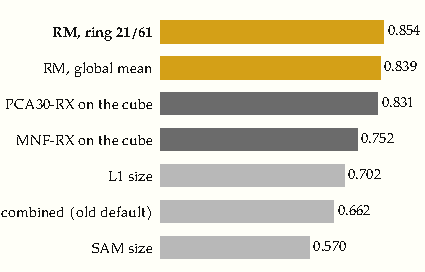
\includegraphics[width=\linewidth]{figures/chart_rm.pdf}
%% src: research/experiments/dual-window-mahalanobis/README.md (mean row, 886 objects)
\take{Scoring the residual's direction, not its size: 0.662 $\to$ 0.854.}
\src{The 21/61 window was the best of four on these same scenes; PCA30-RX still wins Set-3 (0.766 vs 0.749).}
\end{columns}
\end{frame}

%======================================================================
% 10 DETECTION RESULTS
%======================================================================
\begin{frame}{Detection results}
\kicker{labelled PRISMA bench: four scenes, 909 objects, thick cloud excluded}\par\vspace{0.5mm}
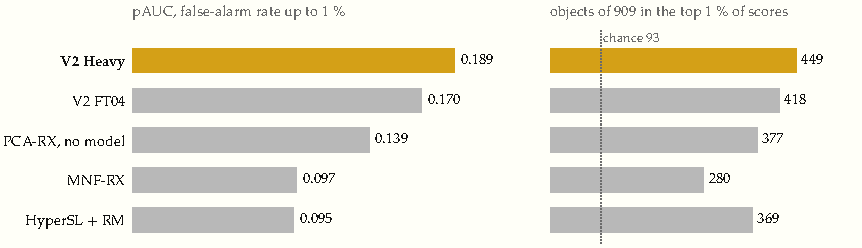
\includegraphics[width=\textwidth]{figures/chart_detection.pdf}
%% src: hypersl-anomaly-bench/README.md (cloud excl.: FTH3 0.1892/449, PCA-RX 0.1390/377, HyperSL RM 0.0947/369, MNF-RX 0.0966/280; chance 10.2% = 93); FT04 0.170 / 46.0% = 418 (FTH3 eval_report.md)
\take{Indradhanu V2 Heavy finds 449 of 909 labelled objects in the top 1\,\% of its scores; the no-model baseline finds 377.}
\vspace{1.5mm}
\begin{columns}[T,onlytextwidth]
\column{0.32\textwidth}
\kicker{against FT04 (paired bootstrap)}\par\vspace{0.3mm}
{\scriptsize pAUC \textbf{+0.0196} [+0.0072, +0.0316]; $P(B>A)=1.000$. Resolved at three neighbouring checkpoints.\par}
%% src: FTH3 bootstrap.txt; README.md (epochs 4/5/6 all resolved)
\column{0.32\textwidth}
\kicker{by difficulty, top 1\,\%}\par\vspace{0.3mm}
{\scriptsize easy 58.2 $\to$ \textbf{62.2}\,\%; medium 39.3 $\to$ \textbf{43.9}\,\%; subtle 40.3 $\to$ \textbf{42.0}\,\%.\par}
%% src: FTH3 README (tiers FT04 -> FTH3 ep5)
\column{0.32\textwidth}
\kicker{product = evaluator}\par\vspace{0.3mm}
{\scriptsize The shipped path reproduces the evaluator's per-scene pAUC to four decimals: 0.2617, 0.1874, 0.0861, 0.2217.\par}
%% src: FTH3 README (product parity table)
\end{columns}
\end{frame}

%======================================================================
% 11 DETECTION DETAIL
%======================================================================
\begin{frame}{Detection detail}
\begin{columns}[T,onlytextwidth]
\column{0.58\textwidth}
\kicker{all measures, 909 objects}\par\vspace{0.3mm}
\fitw{\fontsize{7}{8.4}\selectfont\begin{tabular}{@{}lrrrrr@{}}
\toprule
model & pAUC & top 1\,\% & top 0.1\,\% & ROC & TPR$_{10^{-3}}$\\
\midrule
FT04 & 0.162 & 45.7\,\% & 14.9\,\% & 0.853 & 0.061\\
FT04, cloud excl. & 0.170 & 46.0\,\% & 15.8\,\% & 0.852 & 0.065\\
FTH2 ep 8, thick excl. & 0.186 & 49.0\,\% & 15.7\,\% & 0.870 & 0.066\\
Heavy FTH3 ep 5 & 0.175 & 46.4\,\% & 13.9\,\% & 0.866 & 0.058\\
\rowcolor{ochre!14}\textbf{Heavy FTH3 ep 5, thick excl.} & \textbf{0.189} & \textbf{49.4\,\%} & \textbf{16.0\,\%} & \textbf{0.869} & \textbf{0.065}\\
no model (PCA-RX) & 0.128 & 39.7\,\% & 8.1\,\% & 0.839 & 0.029\\
MNF-RX & 0.075 & 27.4\,\% & 3.4\,\% & 0.749 & 0.019\\
chance & & 10.2\,\% & 1.1\,\% & & \\
\bottomrule
\end{tabular}}\par
%% src: FTH3 eval_report.md (FT04_shipped RM / excl. FT04 masks; FTH2_ep8 excl. FTH2 thick; FTH3_ep5 RM / excl. FTH3_ep5 thick; chance); PCA-RX, MNF-RX from hypersl-anomaly-bench README (no exclusion)
\vspace{2mm}
\kicker{per scene, Heavy FTH3 epoch 5}\par\vspace{0.3mm}
\fitw{\fontsize{7}{8.4}\selectfont\begin{tabular}{@{}lrrrr@{}}
\toprule
& Set-1 & Set-2 & Set-3 & Set-4\\
\midrule
thick cloud excluded & 0.00\,\% & 0.00\,\% & 1.49\,\% & 0.47\,\%\\
pAUC & 0.2617 & 0.1874 & 0.0861 & 0.2217\\
ROC-AUC & 0.9357 & 0.8738 & 0.7807 & 0.8877\\
\bottomrule
\end{tabular}}\par
%% src: FTH3 README (product parity table)
\column{0.38\textwidth}
\kicker{paired bootstrap against FT04}\par\vspace{0.3mm}
\fitw{\fontsize{7}{8.4}\selectfont\begin{tabular}{@{}lll@{}}
\toprule
epoch & pAUC difference & top 0.1\,\%\\
\midrule
4 & +0.0148 [+0.0029, +0.0259] & $-$0.4 pts\\
\textbf{5} & \textbf{+0.0196 [+0.0072, +0.0316]} & +0.1 pts\\
6 & +0.0179 [+0.0055, +0.0292] & $-$0.3 pts\\
\bottomrule
\end{tabular}}\par
%% src: FTH3 bootstrap.txt
\vspace{2mm}
\begin{itemize}\setlength{\itemsep}{0.4mm}\scriptsize
\item Objects, not pixels, are resampled: 909 with replacement, both models on each draw.
\item The top 0.1\,\% is a tie; the gain is in the broad ranking.
\item Three neighbouring checkpoints all resolve, so the gain is not checkpoint luck.
\end{itemize}
%% src: hypersl-anomaly-bench README (object bootstrap); FTH3 README (top 0.1% ties; three epochs)
\end{columns}
\end{frame}

%======================================================================
% 12 AGAINST HYPERSL
%======================================================================
\begin{frame}{Against HyperSL}
\kicker{same bench, same scorer, same pixels; HyperSL's published checkpoint and code unmodified}\par\vspace{0.5mm}
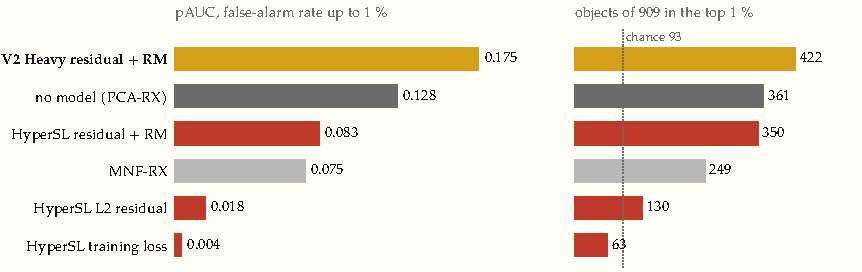
\includegraphics[width=\textwidth]{figures/chart_hypersl.pdf}
%% src: hypersl-anomaly-bench/README.md (Results table, no exclusion; checkpoint unmodified)
\take{HyperSL's reconstruction makes detection worse than using none: 0.083 against 0.128 with no model at all.}
\vspace{1.5mm}
\fitw{\fontsize{7}{8.4}\selectfont\begin{tabular}{@{}lrr@{\hspace{8mm}}lrr@{}}
\toprule
paired difference [95\,\%] & pAUC & top 1\,\% (pts) & & pAUC & top 1\,\% (pts)\\
\midrule
HyperSL $-$ no model & $-$0.045 [$-$0.059, $-$0.032] & $-$1.2 [$-$4.0, +1.5] & no model $-$ V2 & $-$0.047 [$-$0.060, $-$0.033] & $-$6.7 [$-$8.8, $-$4.5]\\
HyperSL $-$ V2 & $-$0.092 [$-$0.106, $-$0.078] & $-$7.9 [$-$10.8, $-$5.2] & same, cloud excluded & $-$0.094 [$-$0.109, $-$0.080] & $-$8.8 [$-$11.7, $-$6.2]\\
\bottomrule
\end{tabular}}\par
%% src: hypersl-anomaly-bench/README.md (difference table: -0.0450 [-0.0589,-0.0318]; -0.0467 [-0.0604,-0.0327]; -0.0917 [-0.1060,-0.0776]; -0.0944 [-0.1094,-0.0800])
\end{frame}

%======================================================================
% 13 WHY NOT HYPERSL
%======================================================================
\begin{frame}{Why not HyperSL}
\begin{columns}[T,onlytextwidth]
\column{0.48\textwidth}
\kicker{1 a pixel rebuilds itself}\par\vspace{0.3mm}
{\scriptsize HyperSL hides bands within a pixel and rebuilds them from that pixel's own visible bands, so an anomaly reconstructs itself. Its own training loss as a score catches 63 objects, below the $\approx$93 of random scores; ROC-AUC 0.501.\par}
\vspace{1.5mm}
\kicker{2 per-scene min-max scaling}\par\vspace{-1mm}
{\footnotesize\[x'_b=\frac{x_b-m_b}{M_b-m_b},\qquad m_b, M_b\ \text{from the scene}\]\par}
\vspace{-1mm}
{\scriptsize The same spectrum (0.20, 0.50) becomes (0.5, 1.0) in one scene and (0.43, 0.75) in another; one bright anomaly rescales every pixel; an angle of 15.07$^\circ$ becomes 36.87$^\circ$. A library spectrum has no scene: 41\,\% of ECOSTRESS values clipped, and a spectrum found its own resampled copy only 28\,\% of the time.\par}
%% src: hypersl-anomaly-bench README (63 objects, ~93, 0.501); docs/training/anomaly-detection/30-min-max-and-the-library.md (toy, 15.07 -> 36.87, 41 %, 28 %)
\column{0.48\textwidth}
\kicker{3 cloud-free pretraining}\par\vspace{0.3mm}
{\scriptsize Same classifier on EnMAP's cloud labels: cirrus recall \textbf{28.9\,\%} from HyperSL features against \textbf{67.9\,\%} from the raw bands. In its favour, thick cloud 87.1\,\% vs 80.4\,\%.\par}
\vspace{1.5mm}
\kicker{4 a smoothing unmixing head}\par\vspace{0.3mm}
\fitw{\fontsize{6.8}{8}\selectfont\begin{tabular}{@{}lrrr@{}}
\toprule
HySU target side (true area, px) & 0.25\,m (0.13) & 0.5\,m (0.51) & 1\,m (2.0)\\
\midrule
ACE, library + field spectra & \textbf{0.97} & \textbf{1.00} & 1.00\\
HyperSL, anchored & 0.68 & 0.77 & 1.00\\
\bottomrule
\end{tabular}}\par
\vspace{1.5mm}
\kicker{the fixes it would need}\par\vspace{0.3mm}
{\scriptsize A fixed normalisation curve, wavelength tokens, whole hidden pixels, clouds in pretraining: the design Indradhanu already has. Not adopted.\par}
%% src: docs/training/anomaly-detection/33-hypersl-cloud-mask.md (28.9 / 67.9; 87.1 / 80.4); 32-hypersl-unmixing.md (0.97 / 1.00 / 1.00; 0.68 / 0.77 / 1.00); 34-hypersl-verdict.md
\end{columns}
\end{frame}

%======================================================================
% 14 CLOUD MASKING
%======================================================================
\begin{frame}{Cloud masking}
\begin{columns}[T,onlytextwidth]
\column{0.36\textwidth}
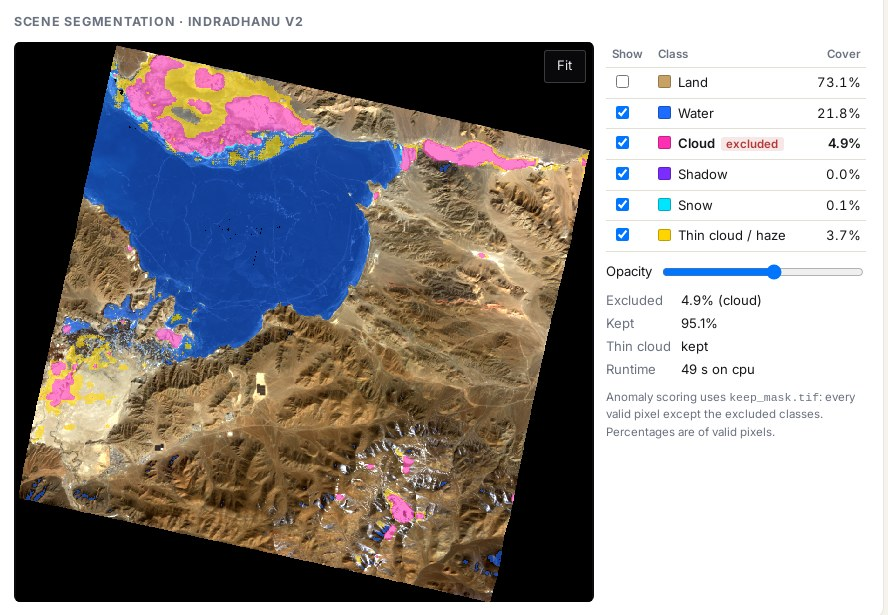
\includegraphics[width=\linewidth]{figures/seg_prisma_panel.jpg}\par
\src{PRISMA, V2 segmentation in the product: land 73.1, water 21.8, cloud 4.9 (left out), thin cloud or haze 3.7, snow 0.1\,\%.}
%% src: screenshot final/seg-prisma_v2.png (product, 2026-11-01)
\column{0.30\textwidth}
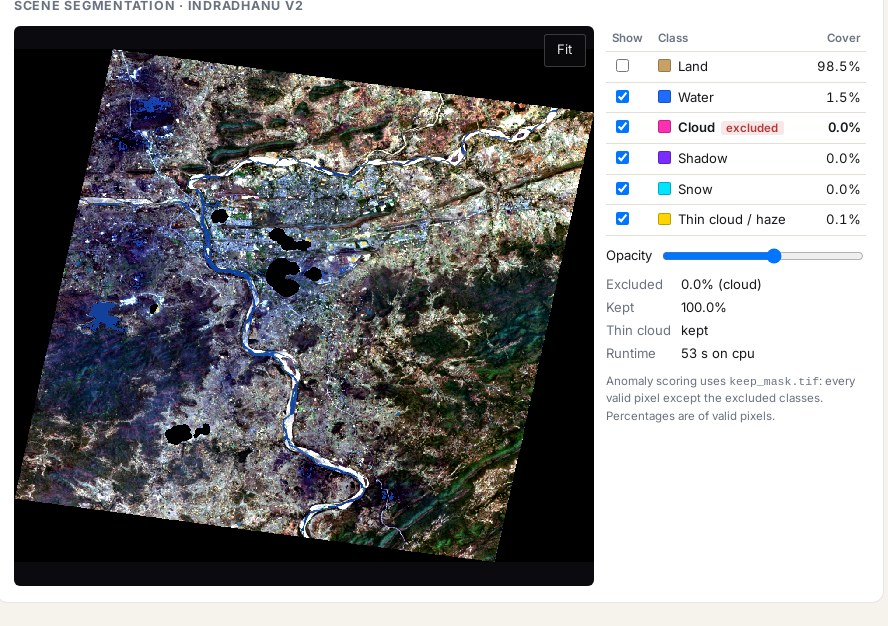
\includegraphics[width=\linewidth]{figures/seg_enmap_panel.jpg}\par
\src{EnMAP, the same step and head.}
\column{0.30\textwidth}
\kicker{the head, validation}\par\vspace{0.3mm}
\fitw{\scriptsize\begin{tabular}{@{}lr@{}}
\toprule
IoU water & 0.825\\
IoU cloud & 0.749\\
IoU thin cloud & 0.090\\
rare classes weighted & $\times$3\\
\bottomrule
\end{tabular}}\par
%% src: FTH3 finetune_metrics.csv epoch 5 (0.8246, 0.7487, 0.0902); config.json (seg_class_weights 3 for shadow, snow)
\vspace{1.5mm}
\kicker{the rule}\par
\begin{itemize}\setlength{\itemsep}{0.3mm}\scriptsize
\item Heavy's thin-cloud output fires on haze: 75.4\,\% of Set-4's pixels and 209 of its 230 targets.
\item So only thick cloud is left out: pAUC 0.175 $\to$ 0.189.
\item Water stays in: vessels are targets.
\end{itemize}
%% src: docs/lld/spectral-stem.md (75.4 %, 209 of 230); eval_report.md (0.175 -> 0.189); docs/lld/segmentation-v2.md (water stays in)
\end{columns}
\end{frame}

%======================================================================
% 15 SPECTRAL NAMER (full-slide schematic)
%======================================================================
\begin{frame}{Spectral namer}
\centering
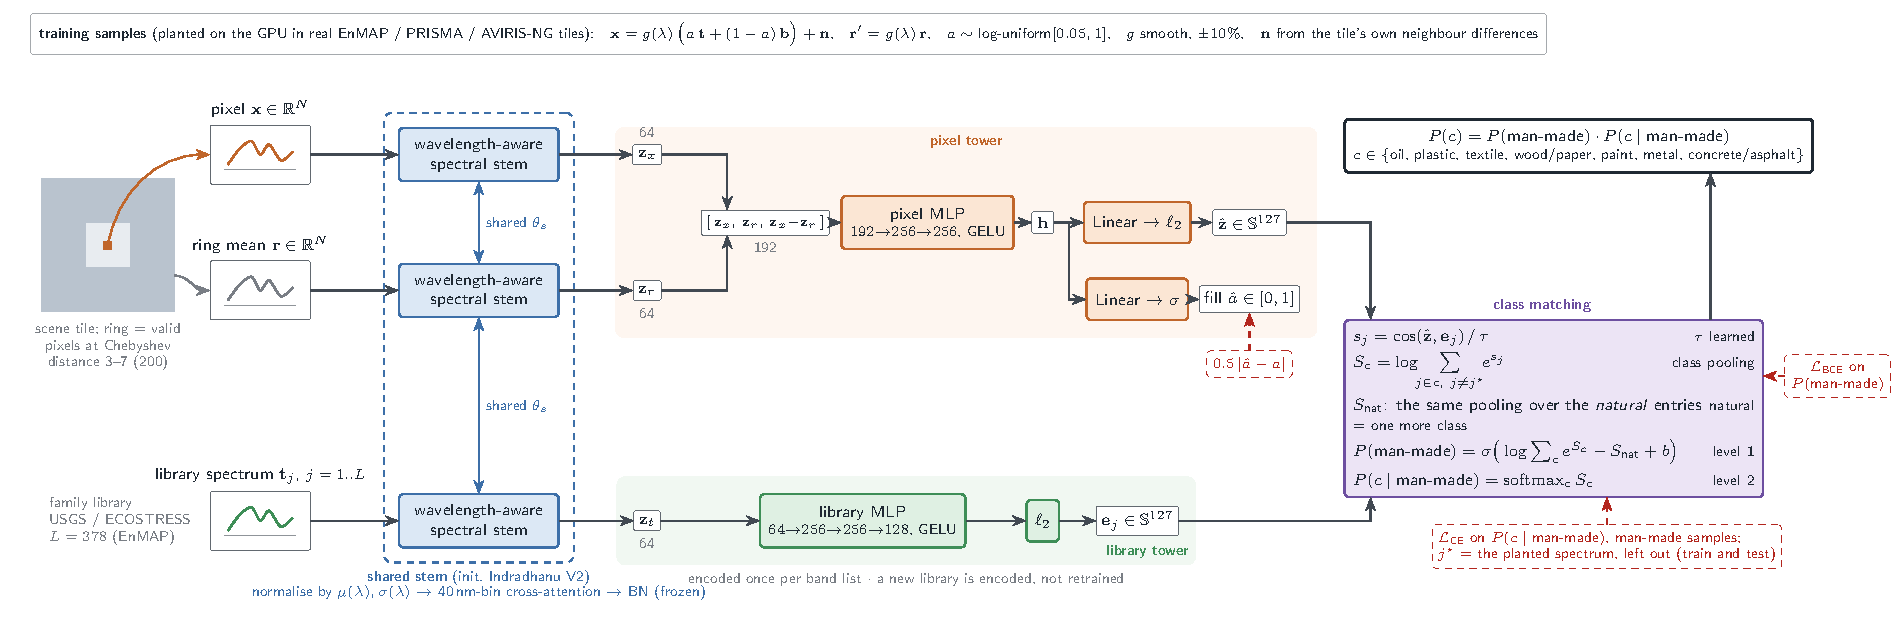
\includegraphics[width=\textwidth,height=0.80\textheight,keepaspectratio]{figures/namer_network.pdf}
\take{Pixel tower and library tower share Indradhanu V2's stem; level 1 (man-made or natural) and level 2 (the class) are both read from the same matching scores.}
%% src: research/experiments/spectral-namer/figures/namer_network.pdf (redrawn 2026-10-31 for level 1 by matching)
\end{frame}

%======================================================================
% 16 NAMER MODEL
%======================================================================
\begin{frame}{Namer model}
\begin{columns}[T,onlytextwidth]
\column{0.48\textwidth}
\kicker{two levels, one set of scores}\par\vspace{-1.5mm}
{\small
\begin{align*}
s_j&=\cos(\mathbf z,\mathbf e_j)/\tau &&\text{library entry } j\\
S_c&=\log\textstyle\sum_{j\in c}e^{s_j} &&\text{class score}\\
\ell&=\operatorname{LSE}(S_0,\dots,S_6)-S_{\text{nat}}+b &&\text{level 1}\\
P(c)&=\sigma(\ell)\cdot\operatorname{softmax}_c(S_c) &&\text{level 2}
\end{align*}\par}
\vspace{-1mm}
{\scriptsize $P(\text{man-made})=\sigma(\ell)$ is the share of the pixel's matching mass on man-made library spectra. $\tau$ is learned. A new library spectrum needs no retraining.\par}
%% src: research/textbook/chapters/42-namer.tex (s_j, class score, level1_logit, share identity); research/experiments/spectral-namer/README.md (P(class) = P(man-made) x P(class|man-made))
\vspace{2mm}
\kicker{classes}\par\vspace{0.3mm}
{\scriptsize oil/fuel, plastic, textile/fabric, wood/paper, paint/coatings, metal, concrete/asphalt; natural spectra form the natural shelf.\par}
\column{0.48\textwidth}
\kicker{trained on planted pixels from real tiles of three sensors}\par\vspace{-1.5mm}
{\footnotesize\[\mathbf x=\mathbf g\odot\big(a\,\mathbf t+(1-a)\,\mathbf b\big)+\mathbf n,\quad a\sim\text{log-uniform}[0.05,1]\]\par}
\vspace{-1.5mm}
{\scriptsize $\mathbf t$ a library spectrum (50\,\% man-made, 25\,\% natural, 25\,\% none), $\mathbf b$ the real background, $\mathbf g$ a smooth gain within $\pm$10\,\%, $\mathbf n$ the tile's own noise.\par}
\vspace{1mm}
{\footnotesize\[\mathcal L=\mathrm{BCE}(\ell,\mathrm M)+\mathrm{CE}(S_{0..6},c)+0.5\,|\hat a-a|\]\par}
\vspace{-1mm}
\fitw{\scriptsize\begin{tabular}{@{}ll@{}}
\toprule
library spectra & 378 / 338 / 380 (EnMAP / PRISMA / AVIRIS-NG)\\
held out & 20\,\% of each man-made class\\
parameters & 347,685, of which the shared stem 17,825\\
optimiser & AdamW $3\!\times\!10^{-4}$, stem at 0.3$\times$\\
run & 40 epochs $\times$ 500 steps on one H100\\
\bottomrule
\end{tabular}}\par
%% src: 42-namer.tex (plant equation, kinds 0.5/0.25/0.25, loss, 347,685, 17,825); N001b README (378/338/380); N001b config.json (a_min 0.05, gain 0.1, lr, stem_lr_scale 0.3, 40 x 500)
\end{columns}
\end{frame}

%======================================================================
% 17 NAMER AGAINST ACE
%======================================================================
\begin{frame}{Namer against ACE}
\begin{columns}[T,onlytextwidth]
\column{0.56\textwidth}
\kicker{level 1: man-made recall at ACE's own natural false-alarm rate}\par\vspace{0.3mm}
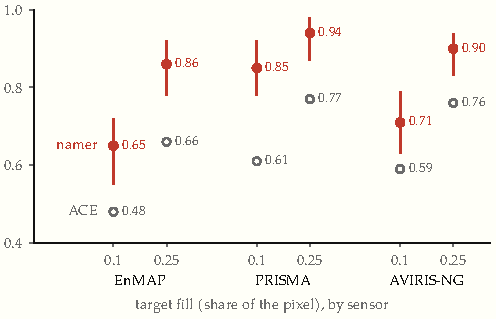
\includegraphics[width=\linewidth]{figures/chart_namer_ace.pdf}
%% src: N001b README "Intervals" table (namer with 95 % CI; ACE point values)
\take{At quarter-pixel fill the namer finds 86--94\,\% of man-made targets; ACE 66--77\,\%.}
\src{Bars: 95\,\% bootstrap over library spectra (221--254 per sensor, 500 draws). ACE: leave-one-spectrum-out.}
\column{0.40\textwidth}
\kicker{level 2: class accuracy on unseen spectra}\par\vspace{0.3mm}
\fitw{\fontsize{6.8}{8}\selectfont\begin{tabular}{@{}lll@{}}
\toprule
sensor, fill & namer [95\,\%] & ACE\\
\midrule
EnMAP 0.1 & \textbf{0.59} [0.48, 0.70] & 0.24\\
EnMAP 0.25 & \textbf{0.68} [0.55, 0.79] & 0.47\\
PRISMA 0.1 & \textbf{0.69} [0.53, 0.81] & 0.41\\
PRISMA 0.25 & 0.70 [0.54, 0.82] & 0.60\\
AVIRIS-NG 0.1 & \textbf{0.65} [0.53, 0.76] & 0.38\\
AVIRIS-NG 0.25 & 0.70 [0.57, 0.82] & 0.58\\
\bottomrule
\end{tabular}}\par
%% src: N001b README "Intervals" table
\vspace{1.5mm}
\kicker{the open set (textile held out)}\par
\begin{itemize}\setlength{\itemsep}{0.3mm}\scriptsize
\item Unseen textile: called man-made 46--47\,\%; then a confident wrong class 45--46\,\%.
\item Abstention sends only 1--4\,\% to ``unknown''.
\item On known classes the flag works: 0.80 / 0.84 / 0.81 accurate at 90\,\% coverage. The product says ``closest known class''.
\end{itemize}
%% src: research/experiments/spectral-namer/N002/README.md
\end{columns}
\end{frame}

%======================================================================
% 18 ATMOSPHERIC CORRECTION
%======================================================================
\begin{frame}{Atmospheric correction}
\centering
\resizebox{\textwidth}{!}{%
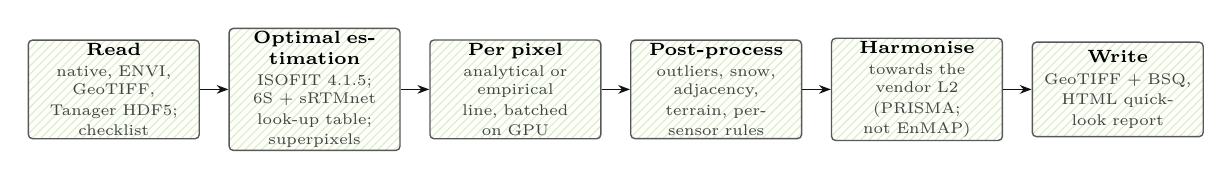
\begin{tikzpicture}[x=1mm,y=1mm]
\foreach \i/\t/\b in {
 {0/Read/native, ENVI, GeoTIFF,\\Tanager HDF5; checklist},
 {1/Optimal estimation/ISOFIT 4.1.5; 6S + sRTMnet\\look-up table; superpixels},
 {2/Per pixel/analytical or empirical\\line, batched on GPU},
 {3/Post-process/outliers, snow, adjacency,\\terrain, per-sensor rules},
 {4/Harmonise/towards the vendor L2\\(PRISMA; not EnMAP)},
 {5/Write/GeoTIFF + BSQ,\\HTML quick-look report}}{
  \node[stg, pattern color=pG!90, minimum width=21mm, minimum height=12mm, text width=21mm] (a\i) at (\i*25.5,0) {\textbf{\upshape\t}\\[0.4mm]{\upshape\color{ink!80}\fontsize{5.6}{6.6}\selectfont \b}};}
\foreach \i [evaluate=\i as \j using int(\i+1)] in {0,...,4} \draw[df] (a\i.east) -- (a\j.west);
\end{tikzpicture}}
%% src: C:/wt/atm-docker/isofit-atm-docker/README.md (stages read -> ISOFIT -> post-process -> harmonise -> write -> report; batched per-pixel solve)
\take{One offline container turns L1 radiance into L2 surface reflectance for EnMAP, PRISMA, AVIRIS-NG, Tanager and GHOSt.}
\vspace{1.5mm}
\begin{columns}[T,onlytextwidth]
\column{0.56\textwidth}
\kicker{end-to-end trials of the shipped container}\par\vspace{0.3mm}
\fitw{\fontsize{6.8}{8}\selectfont\begin{tabular}{@{}llrr@{}}
\toprule
scene & reference & time & land MAE\\
\midrule
PRISMA, Maharashtra coast & ASI L2C & 33 min & 0.0124\\
Tanager, Thessaloniki & Planet SR & 36 min & 0.0114\\
Tanager, ROCX2025 & Planet SR & 44 min & 0.0089\\
PRISMA, Himachal, 18.5\,\% snow & ASI L2D & 26 min & 0.0461\\
EnMAP, Sundarbans, haze & DLR L2A & 33 min & 0.0157\\
Tanager, Permian, gas flares & Planet SR & 36 min & 0.0092\\
\rowcolor{ochre!14}AVIRIS-NG full line, 4.0 Mpix & JPL & \textbf{41 min} & \textbf{0.0057}\\
\bottomrule
\end{tabular}}\par
%% src: C:/wt/atm-docker/research/experiments/atm-correction/EXPERIMENT_LOG.md AC26-T11 (T1-T6 core land MAE, times) and AC26-T7B (41 min, 0.0057)
\column{0.40\textwidth}
\kicker{held-out accuracy}\par
\begin{itemize}\setlength{\itemsep}{0.3mm}\scriptsize
\item PRISMA, five unseen scenes against ASI: land MAE 0.0244 $\to$ \textbf{0.0099} after harmonisation.
\item EnMAP against DLR: 0.0098 already; harmonisation did not help, so it is off.
\item AVIRIS-NG against JPL: bias +0.0031, median spectral angle 2.27$^\circ$.
\end{itemize}
%% src: EXPERIMENT_LOG.md AC26-HON (0.0244 -> 0.0099; EnMAP 0.0098 -> 0.0100); AC26-T7B (+0.0031, 2.27 deg)
\vspace{1mm}
\kicker{the product}\par
{\scriptsize Reflectance $\times$10,000 as 16-bit integers, no-data $-$9999, water-vapour bands dropped and listed, wavelengths and FWHM in both files; outlier, snow and provenance sidecars.\par}
%% src: isofit-atm-docker/README.md
\end{columns}
\end{frame}

%======================================================================
% 19 ANY SENSOR
%======================================================================
\begin{frame}{Any sensor}
\begin{columns}[T,onlytextwidth]
\column{0.60\textwidth}
\fitw{\fontsize{6.8}{8}\selectfont\begin{tabular}{@{}>{\raggedright}p{14mm}>{\raggedright}p{27mm}>{\raggedright}p{20mm}>{\raggedright\arraybackslash}p{27mm}@{}}
\toprule
sensor & input & map grid from & checked\\
\midrule
PRISMA & L2D HE5, native bands & the file's UTM corners & ground-truth grid reproduced exactly\\
EnMAP & L2A, 224 bands & vendor GeoTIFF & segmentation and scoring end to end\\
AVIRIS-NG & ENVI, 372 bands & ENVI map info & 2,375 objects on the match screen\\
Tanager & HDF5 or ENVI; 426 bands, 368 good & HDF-EOS grid & UTM 13N, 30\,m\\
any HSI file & GeoTIFF, ENVI, HDF5, NetCDF & file CRS or geolocation file & pre-flight report: bands, FWHM, scale, no-data\\
\bottomrule
\end{tabular}}\par
%% src: docs/proposals/aigc-evaluation-submission.md (C1); docs/lld/tanager.md (426 / 368, EPSG:32613, 30 m); docs/lld/generic-hsi.md; FTH3 config (EnMAP 224, AVIRIS-NG 372); spectral-namer-in-product.md (2,375)
\vspace{2mm}
\kicker{the PRISMA georeference fix}\par\vspace{-1.5mm}
{\footnotesize\[
\mathbf A=\begin{pmatrix}d_x&0&U\!L_e-\tfrac{d_x}{2}\\0&-d_y&U\!L_n+\tfrac{d_y}{2}\end{pmatrix},\quad
d_x=\frac{U\!R_e-U\!L_e}{W-1},\ d_y=\frac{U\!L_n-L\!L_n}{H-1}
\]\par}
\vspace{-1.5mm}
{\scriptsize The corners are pixel centres. The old latitude/longitude box fit was a median \textbf{2.4\,px} off (95th percentile 4.1, max 5.6). Internal evaluation was never affected: it works in pixel space.\par}
%% src: docs/proposals/aigc-evaluation-submission.md (2.4 px median, 95 % 4.1, max 5.6; affine)
\vspace{1mm}
{\scriptsize V2 reads every band within 15\,nm of the 733 wavelengths it was trained on: all 185 of PRISMA's.\par}
%% src: research/textbook/chapters/41-heavy.tex (trained_wl 733; 185 kept)
\column{0.37\textwidth}
\setlength{\tabcolsep}{0.6mm}
\begin{tabular}{@{}cc@{}}
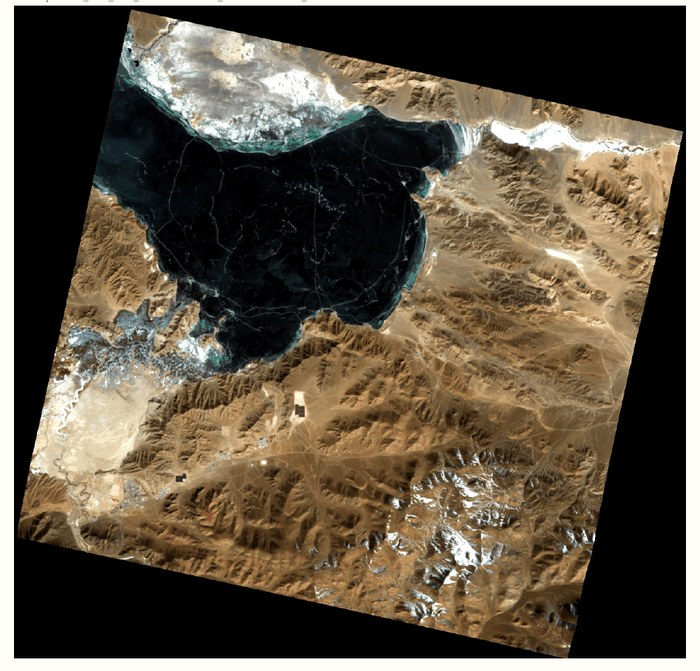
\includegraphics[height=27mm]{figures/story_prisma_k1.jpg}&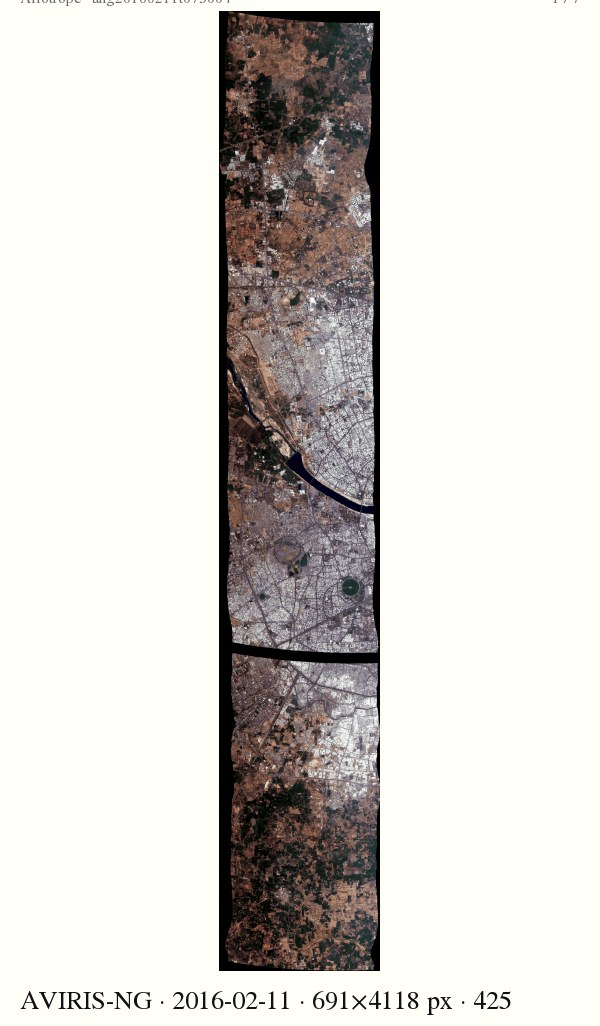
\includegraphics[height=27mm]{figures/story_aviris_k1.jpg}\\[-0.6mm]
\srcc{PRISMA}&\srcc{AVIRIS-NG}\\
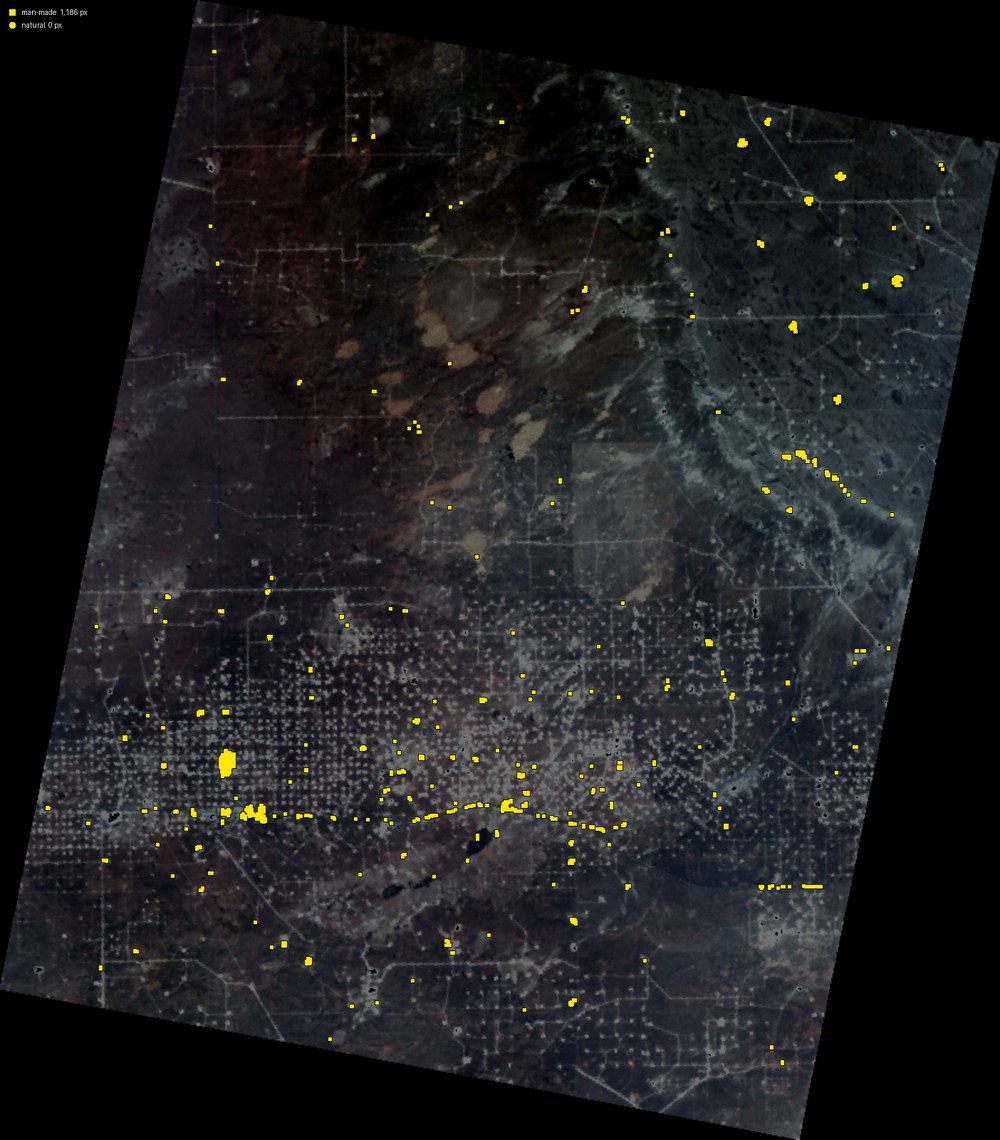
\includegraphics[height=27mm]{figures/ql_tanager_manmade.jpg}&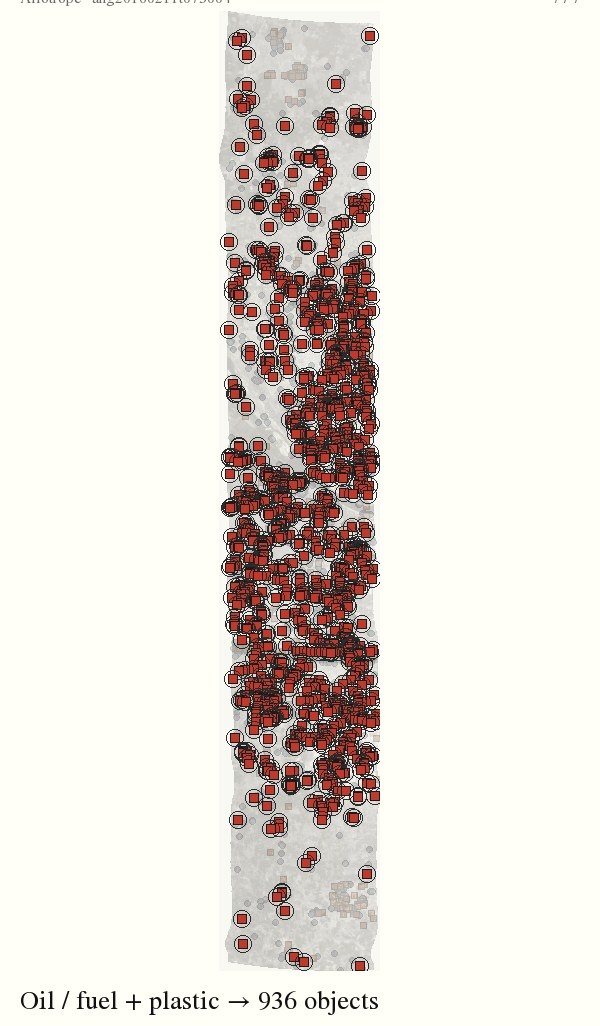
\includegraphics[height=27mm]{figures/story_aviris_k7.jpg}\\[-0.6mm]
\srcc{Tanager, man-made}&\srcc{AVIRIS-NG, oil + plastic}
\end{tabular}
\end{columns}
\end{frame}

%======================================================================
% 20 DELIVERABLES
%======================================================================
\begin{frame}{Deliverables}
\begin{columns}[T,onlytextwidth]
\column{0.40\textwidth}
\kicker{per scene and selection}\par\vspace{0.6mm}
\fitw{\fontsize{6.8}{8.2}\selectfont\begin{tabular}{@{}>{\ttfamily}l>{\raggedright\arraybackslash}p{24mm}@{}}
\toprule
\rmfamily file & content\\
\midrule
hyper\_anomaly\_mask\_<sel>.tif & boolean mask, 0/1\\
hyper\_anomaly\_pixels\_<sel>.shp & one point per pixel\\
hyper\_anomaly\_objects\_<sel>.shp & one point per object\\
hyper\_anomaly\_objects\_<sel>.csv & the same, as a table\\
hyper\_quicklook\_<sel>.png & RGB with the selection\\
MANIFEST.json & every choice in the chain\\
<scene>\_L2\_SR.tif / .bsq & surface reflectance\\
\bottomrule
\end{tabular}}\par
%% src: docs/lld/spectral-namer-in-product.md (class-driven pack); C:/wt/atm-docker/isofit-atm-docker/README.md (L2_SR)
\vspace{2mm}
\kicker{mask GeoTIFF, PRISMA example}\par\vspace{0.3mm}
\fitw{\scriptsize\begin{tabular}{@{}ll@{}}
\toprule
CRS & UTM zone 44N (EPSG:32644)\\
pixel & 30 m, origin 375472.78 E, 3721282.25 N\\
values & 8-bit, 0 or 1, no no-data value\\
man-made pack & 110 objects, 865 pixels\\
\bottomrule
\end{tabular}}\par
%% src: docs/lld/spectral-namer-in-product.md (class-driven e2e: EPSG:32644 (30, 0, 375472.78, 0, -30, 3721282.25); classes=manmade 110 / 865)
\column{0.33\textwidth}
\kicker{shapefile attributes}\par\vspace{0.3mm}
\fitw{\fontsize{6.8}{8.2}\selectfont\begin{tabular}{@{}>{\ttfamily}l>{\raggedright\arraybackslash}p{30mm}@{}}
\toprule
lat, lon & WGS84 degrees\\
nm\_call & man-made or natural\\
nm\_mm & object's $P(\text{man-made})$\\
nm\_cls & closest known class\\
nm\_p & $P(\text{class}\mid\text{man-made})$\\
nm\_conf & 1 confident, 0 tentative\\
family & ACE family match\\
mat1, scr1 & best SAM library match, angle\\
\bottomrule
\end{tabular}}\par
%% src: docs/lld/spectral-namer-in-product.md (pixel shapefile columns); confident at P >= 0.55 (N002 README)
\vspace{1.5mm}
{\scriptsize The object table adds the object id, pixel count and centroid.\par}
\column{0.23\textwidth}
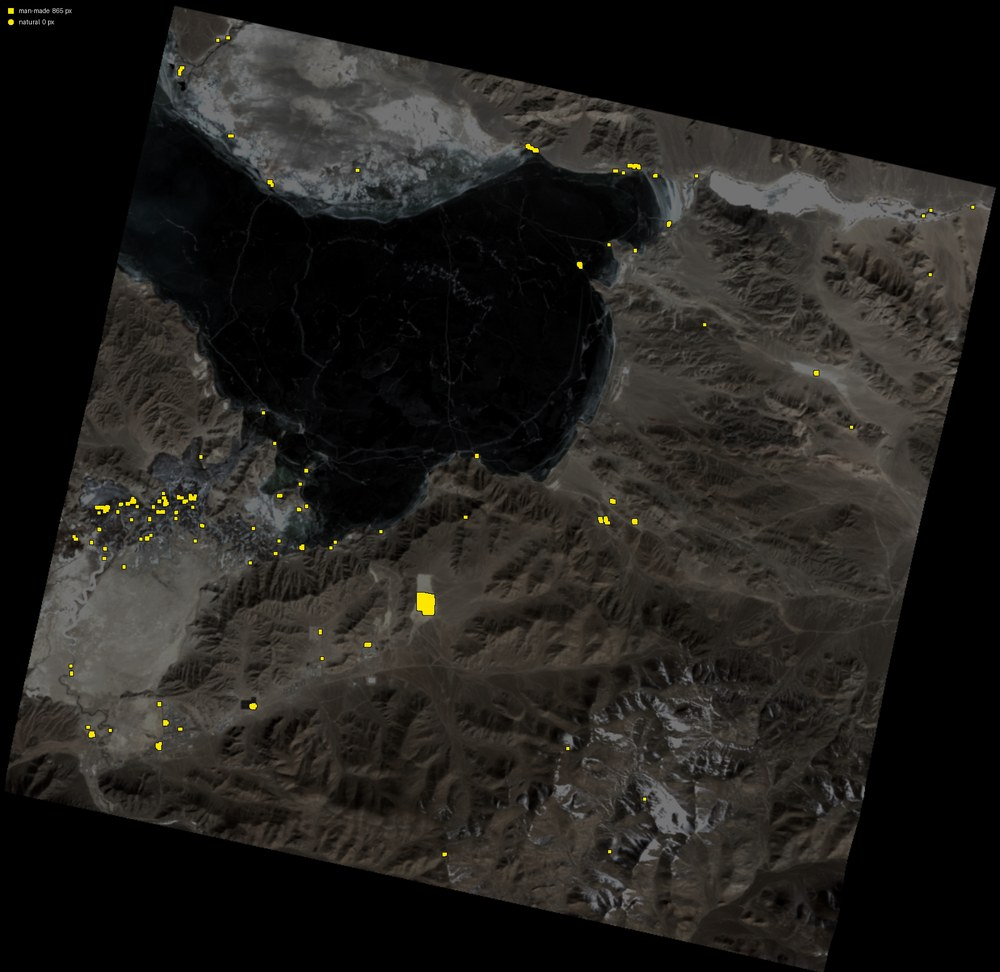
\includegraphics[width=\linewidth]{figures/ql_prisma_manmade.jpg}\par
\src{Quick-look: selected pixels in yellow, squares man-made, circles natural.}
\end{columns}
\end{frame}

%======================================================================
% 21 PRODUCT
%======================================================================
\begin{frame}{Product}
\begin{columns}[T,onlytextwidth]
\column{0.60\textwidth}
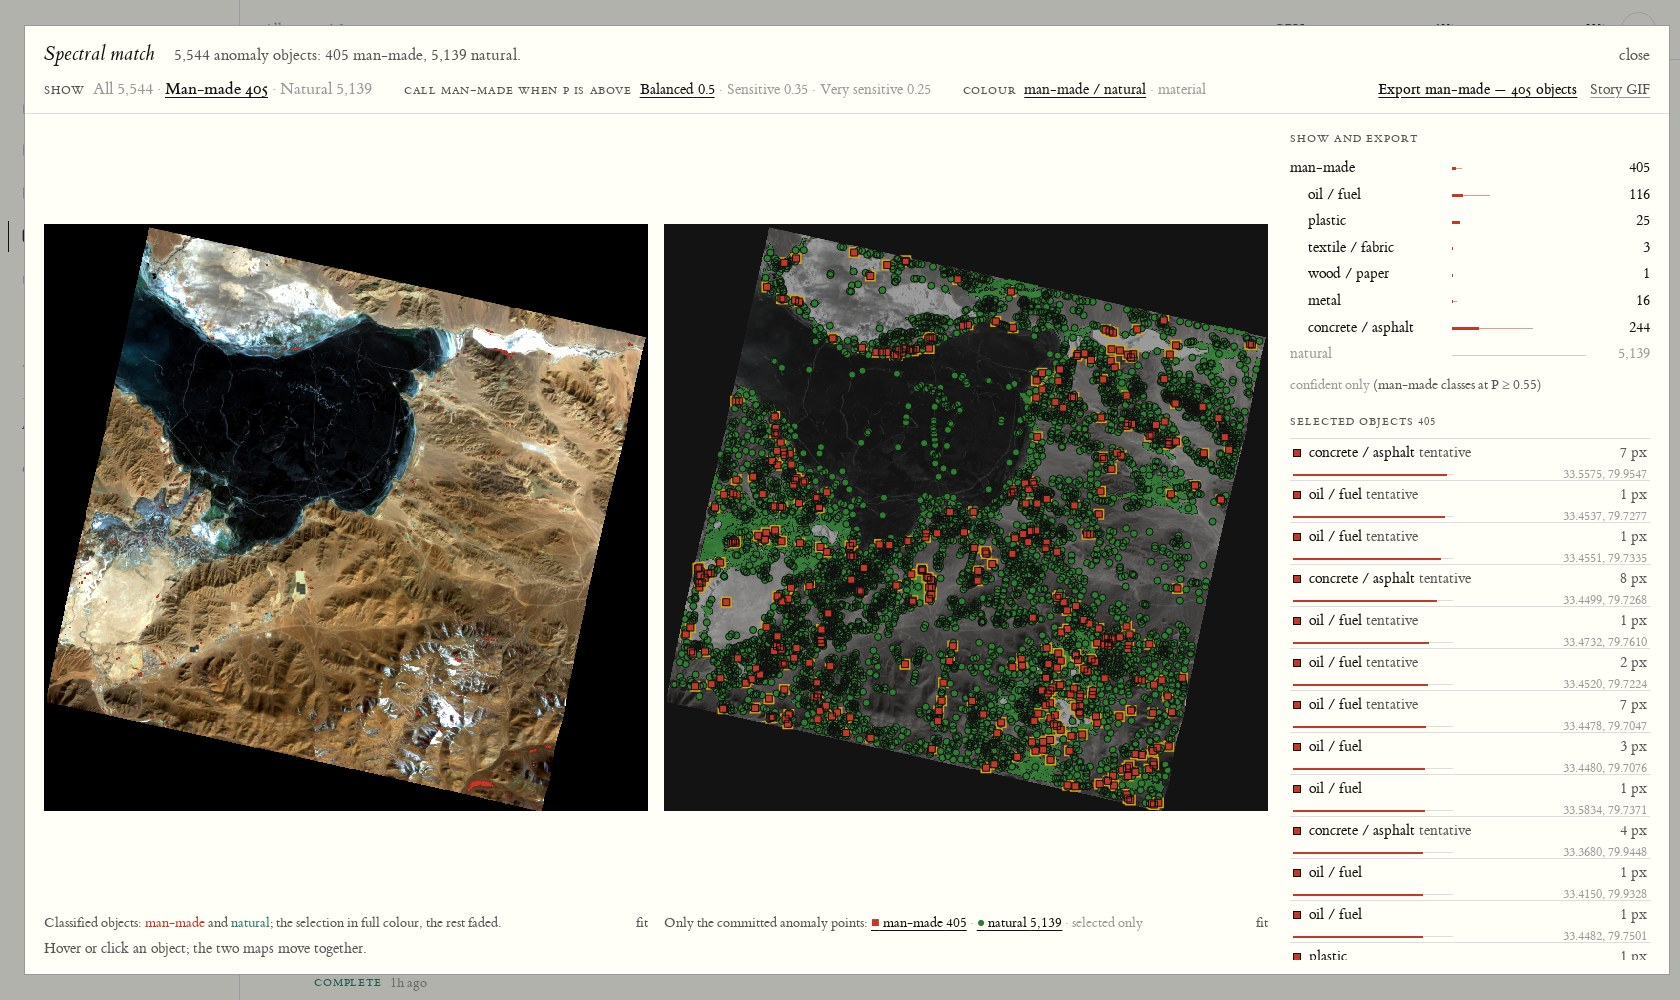
\includegraphics[width=\linewidth]{figures/match_prisma.jpg}\par
\src{Match screen: classified map and anomaly points, pan and zoom linked; man-made and natural, material classes, three sensitivity presets; the export button names the selection.}
%% src: scratchpad final/flowB/prisma-1-open.png; docs/proposals/class-driven-flow.md (additions A, D)
\column{0.37\textwidth}
\kicker{class-driven export, end to end}\par\vspace{0.3mm}
\fitw{\fontsize{6.8}{8.2}\selectfont\begin{tabular}{@{}lrr@{}}
\toprule
objects / mask pixels & PRISMA & Tanager\\
\midrule
committed pixels & 7,435 & 4,565\\
man-made & 110 / 865 & 272 / 1,186\\
oil/fuel + plastic & 26 / 598 & 247 / 1,124\\
natural & 852 / 6,570 & 831 / 3,379\\
man-made, sensitive 0.35 & 240 / 1,672 & 424 / 2,073\\
\bottomrule
\end{tabular}}\par
%% src: docs/lld/spectral-namer-in-product.md (class-driven flow e2e table)
\src{Every pack checked: values 0/1, mask pixels and table rows equal the selection, shapefiles open in the scene CRS.}
\vspace{1mm}
\begin{itemize}\setlength{\itemsep}{0.3mm}\scriptsize
\item Classes to leave out are chosen at scoring, from V2's class map.
\item A story GIF shows the seven-step narrowing; it never enters a pack.
\item Runs on an air-gapped GPU server from an offline update kit that keeps all data.
\end{itemize}
%% src: docs/proposals/class-driven-flow.md (gap 1); docs/lld/story-gif.md; docker/airgap-update/README.md
\end{columns}
\end{frame}

%======================================================================
% 22 SUMMARY
%======================================================================
\begin{frame}{Summary}
\fitw{\fontsize{7.6}{9.4}\selectfont\begin{tabular}{@{}>{\raggedright}p{52mm}>{\raggedright\arraybackslash}p{88mm}@{}}
\toprule
claim & evidence\\
\midrule
Indradhanu V2 Heavy is our best detector & pAUC 0.189 vs FT04 0.170, +0.0196 [+0.0072, +0.0316]; 449 of 909 objects in the top 1\,\%\\
the model adds over no model & +0.047 pAUC over PCA-RX on the same scorer\\
HyperSL is not adopted & 0.083 with its reconstruction, below 0.128 with none\\
the namer separates man-made from natural better than ACE & +0.20 / +0.17 / +0.14 recall at ACE's false-alarm rate, quarter-pixel fill\\
it names small targets better than ACE & class accuracy 0.59--0.69 against 0.24--0.41 at 10\,\% fill\\
L2 reflectance from L1, offline & 0.0057 vs JPL on AVIRIS-NG; PRISMA 0.0099 vs ASI on unseen scenes\\
georeferenced, heatmap-free packs & the scene's own UTM grid; the 2.4-pixel PRISMA offset fixed\\
any sensor & PRISMA, EnMAP, AVIRIS-NG, Tanager, GHOSt and any GeoTIFF, ENVI or HDF5 cube\\
\bottomrule
\end{tabular}}\par
%% src: as on the detection, HyperSL, namer, atmospheric-correction and sensor slides (FTH3 README/bootstrap; hypersl-anomaly-bench README; N001b README; EXPERIMENT_LOG AC26-T7B/AC26-HON; aigc-evaluation-submission.md)
\end{frame}

%======================================================================
% 23 LIMITS AND NEXT
%======================================================================
\begin{frame}{Limits and next}
\begin{columns}[T,onlytextwidth]
\column{0.55\textwidth}
\kicker{honest limits}\par
\begin{itemize}\setlength{\itemsep}{0.8mm}\small
\item \textbf{Open set.} An unseen material gets the nearest of seven classes; abstention catches 1--4\,\%.
\item \textbf{Solar panels.} In-scene PV spectra added to the library changed nothing ($P(\text{man-made})$ 0.248 $\to$ 0.248); they need lab spectra or a retrain.
\item \textbf{Calibration.} The 0.5 man-made call is not scene-calibrated; Tanager was not a training sensor.
\item \textbf{Bench size.} Four labelled PRISMA scenes; resolution about $\pm$0.005--0.01 pAUC.
\item \textbf{Cost.} Heavy is 1.7$\times$ FT04 on CPU: 454 vs 274\,s per scene.
\item \textbf{Thermal.} The chain is built (Chakshu) but no thermal scene has run on this stack.
\end{itemize}
%% src: N002 README; pv-library README; spectral-namer-in-product.md gotcha 5; docs/lld/evaluation.md; FTH3 README; aigc-evaluation-submission.md R3
\column{0.41\textwidth}
\kicker{next}\par
\begin{itemize}\setlength{\itemsep}{0.8mm}\small
\item Library augmentation for level 2 (run N003), swapped in without code changes.
\item Field spectra for camouflage and military coatings; a glass and solar-panel class.
\item A larger labelled bench, beyond PRISMA.
\end{itemize}
%% src: N003 README (results pending); spectral-namer-in-product.md ("N003 replaces it by a manifest edit"); spectral-namer README (class list)
\end{columns}
\end{frame}

%======================================================================
% 24 OUR JOURNEY
%======================================================================
\begin{frame}{Our journey}
\centering
\resizebox{\textwidth}{!}{%
\begin{tikzpicture}[x=1mm,y=1mm, every node/.append style={execute at begin node={\hyphenpenalty=10000\exhyphenpenalty=10000}}]
% phase bands (x is piecewise: Jan-Aug compressed, October expanded; breaks drawn on the axis)
\fill[band] (-1,-31) rectangle (34,25);
\fill[band!55] (34.6,-31) rectangle (60,25);
\fill[band] (60.6,-31) rectangle (121,25);
\fill[band!55] (121.6,-31) rectangle (149,25);
\foreach \x/\t in {16.5/Foundation, 47.3/Product, 90.8/Detection, 135.3/Material}
  \node[font=\scshape\fontsize{6.6}{7}\selectfont, color=mute] at (\x,22.8) {\t};
% axis
\draw[ink, line width=0.4pt] (-1,0) -- (149,0);
\foreach \x/\d in {0/Jan,10/Mar,20/Apr,30/May,36/Jul,48/Aug,62/14 Oct,80/19 Oct,98/22 Oct,112/29 Oct,128/31 Oct,146/1 Nov}
  {\draw[ink] (\x,0) -- (\x,-0.9); \node[font=\fontsize{5.6}{6}\selectfont, color=mute, below] at (\x,-0.9) {\d};}
\foreach \b in {34.3,60.3} {\fill[band] (\b-0.9,-1.2) rectangle (\b+0.9,1.2);
  \draw[ink] (\b-1.4,-1.2) -- (\b-0.4,1.2); \draw[ink] (\b+0.4,-1.2) -- (\b+1.4,1.2);}
% milestones (above)
\foreach \x/\h/\w/\t in {
 {0/12/17mm/{\textbf{26 Jan} first\\commit: HE5 and\\TIF readers}},
 {10/4/9mm/{\textbf{23 Mar}\\first\\trainer}},
 {20/12/13mm/{\textbf{10 Apr}\\hyperspectral\\SegFormer MAE}},
 {36/4/22mm/{\textbf{23 Jul} backend +\\frontend: the app}},
 {62/12/17mm/{\textbf{14 Oct} Spectral-\\Earth pretraining,\\wavelength stem}},
 {66/3/13mm/{\textbf{15 Oct}\\residual\\Mahalanobis}},
 {80/12/17mm/{\textbf{19 Oct} FT04\\ships as V2,\\pAUC 0.170}},
 {106/12/18mm/{\textbf{28--29 Oct}\\Heavy on an H100:\\0.189, v2.1.0}},
 {128/12/13mm/{\textbf{31 Oct}\\namer N001b\\passes level 1}}}
 {\draw[ink, line width=0.35pt] (\x,0) -- (\x,\h); \fill[ink] (\x,0) circle (0.7); \node[ms=\w] at (\x+0.6,\h-0.6) {\t};}
\draw[ochre, line width=0.6pt] (146,0) -- (146,4); \fill[ochre] (146,0) circle (1.1);
\node[font=\fontsize{7}{8}\selectfont, anchor=south east, align=right] at (148,4.3) {\textbf{v1.0}};
% failures (below): x, level, width, text
\foreach \x/\h/\w/\t in {
 {30/-5/17mm/{\textbf{May} plain RX\\fails: covariance\\near singular,\\distances $10^{11}$\\$\to$ MNF-RX}},
 {48/-5/12.5mm/{\textbf{Aug} two\\outages hit\\main; fake\\docs removed\\$\to$ check\\the worker}},
 {98/-5/13mm/{\textbf{22 Oct} FT07,\\FT08: 0.165,\\0.164 $<$ 0.170\\$\to$ widen\\the model}},
 {112/-5/11mm/{\textbf{29 Oct}\\haze read\\as cloud:\\209 of 230\\targets $\to$\\thick only}},
 {124/-17/13mm/{\textbf{31 Oct}\\HyperSL:\\0.083 $<$ 0.128\\$\to$ rejected}},
 {130/-5/13mm/{\textbf{31 Oct}\\N001 level 1\\at chance\\(0.50) $\to$\\matching}}}
 {\draw[manmade!60, line width=0.35pt] (\x,-3.3) -- (\x,\h); \draw[manmade, line width=0.5pt] (\x-0.7,-0.7) -- (\x+0.7,0.7) (\x-0.7,0.7) -- (\x+0.7,-0.7); \node[fl=\w] at (\x+0.6,\h+0.6) {\t};}
\draw[manmade!60, line width=0.35pt] (146,-3.3) -- (146,-17);
\draw[manmade, line width=0.5pt] (145.3,-0.7) -- (146.7,0.7) (145.3,0.7) -- (146.7,-0.7);
\node[fl=10mm, anchor=north east, align=right] at (147.5,-17.6) {\textbf{1 Nov}\\PV spectra:\\no effect};
% pAUC sparkline (matplotlib, figures/chart_spark.pdf)
\node[anchor=south west, inner sep=0] at (63,-30) {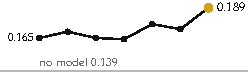
\includegraphics[width=42mm]{figures/chart_spark.pdf}};
\node[font=\fontsize{5.6}{6}\selectfont, color=mute, anchor=north west] at (64,-30.3) {pAUC: v0.2.0, FT04, FT07, FT08, FT09b, FT09c, Heavy};
\end{tikzpicture}}

%% src dates: git log (3625df1 2026-01-26; 727e3e4 2026-03-23; d2f8c3c 2026-04-10; 0cc4335 2026-07-23; c002970/392e106 2026-10-14; 4b7da29 2026-10-15; 20afa70 2026-10-19; 8c14fe6 2026-10-22; a0b6930 2026-10-28; c4b3a63 2026-10-29; 0c2efe8 2026-10-31; 53ac8d7 2026-11-01)
%% src failures: CLAUDE.md (plain RX dropped 2026-05-11, distances 1e11; two outages; docs/tech fabricated, removed 2026-08-24); docs/lld/evaluation.md (FT07/FT08 0.165/0.164 vs 0.170); docs/lld/spectral-stem.md (209 of 230); hypersl-anomaly-bench README (0.083 vs 0.128); N001 README (0.50 at fill 1.0); pv-library README
\vspace{0.3mm}
{\small From a pipeline to a product: \textbf{any sensor in, georeferenced answers out.}\hfill{\color{mute}\footnotesize Allotrope v1.0 \textperiodcentered{} 1 November 2026}}
\end{frame}

%======================================================================
% APPENDIX
%======================================================================
\appendix
\renewcommand{\decklabel}{Allotrope v1.0 \textperiodcentered{} AIGC Stage III \textperiodcentered{} appendix}

\begin{frame}{A1 Heavy training}
\begin{columns}[T,onlytextwidth]
\column{0.50\textwidth}
\kicker{pretraining on SpectralEarth, 202 bands}\par\vspace{0.3mm}
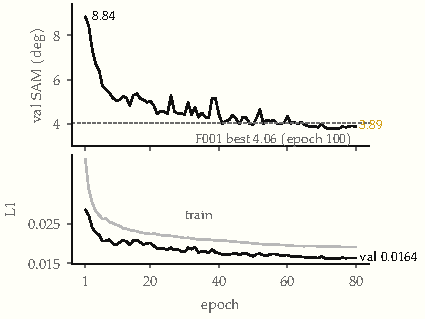
\includegraphics[width=\linewidth]{figures/chart_f002.pdf}
%% src: F002-heavy/metrics.csv (plotted); README.md (8.84 at epoch 1; 0.0164 / 3.89 at 80; F001 best 4.06 at 100)
\take{80 epochs; validation SAM 3.89$^\circ$, below F001's best of 113 epochs.}
\column{0.46\textwidth}
\kicker{run}\par\vspace{0.3mm}
\fitw{\fontsize{6.8}{8.2}\selectfont\begin{tabular}{@{}ll@{}}
\toprule
hardware & one H100 80\,GB, rented capacity block\\
throughput & 369\,s per epoch, 81.2 patches/s, 18.4\,GB\\
data & 3,200 of 3,419 shards, 30,000 patches per epoch\\
best checkpoint & epoch 72\\
\bottomrule
\end{tabular}}\par
%% src: F002-heavy README (369 s, 81.2, 18.4 GB, 3,200 of 3,419, best.pt epoch 72); config.json (30,000)
\vspace{1.5mm}
\kicker{parameters}\par\vspace{0.3mm}
\fitw{\fontsize{6.8}{8.2}\selectfont\begin{tabular}{@{}lrr@{}}
\toprule
part & FT04 & Heavy\\
\midrule
spectral stem & 14,721 & 17,825\\
encoder & 3,331,072 & 29,580,288\\
decoder & 2,164,736 & 4,279,616\\
output layer + norm & 4,321 & 6,465\\
segmentation head & & 1,431,120\\
\midrule
served & 5.9\,M & \textbf{35,315,314}\\
\bottomrule
\end{tabular}}\par
%% src: research/textbook/chapters/41-heavy.tex (whole-model counts; served total); docs/04-models.md (FT04 5.9 M)
\vspace{1.5mm}
\kicker{pretrained only, no fine-tuning}\par\vspace{0.3mm}
\fitw{\fontsize{6.8}{8.2}\selectfont\begin{tabular}{@{}lrr@{}}
\toprule
& pAUC & top 1\,\% / 0.1\,\%\\
\midrule
F001, FT04 size & 0.155 & 45.1 / 14.0\,\%\\
F002 Heavy & 0.166 & 47.4 / 12.4\,\%\\
\bottomrule
\end{tabular}}\par
%% src: F002-heavy README (Detection, pretrained only)
\end{columns}
\end{frame}

\begin{frame}{A2 Namer runs}
\begin{columns}[T,onlytextwidth]
\column{0.56\textwidth}
\fitw{\fontsize{6.8}{8.2}\selectfont\begin{tabular}{@{}l>{\raggedright}p{26mm}>{\raggedright\arraybackslash}p{44mm}@{}}
\toprule
run & change & result\\
\midrule
N001 & linear level-1 head & stopped after epoch 1: level 1 at chance, 0.49--0.52 (0.50 at full fill, where ACE gets 0.87)\\
N001b & level 1 by matching & passes on all three sensors, +0.20 / +0.17 / +0.14; \textbf{served, epoch 40}\\
N002 & textile held out & open set fails: 0.46--0.47 called man-made\\
N003 & library augmentation & results pending\\
PV library & 50 in-scene PV spectra & no effect, 0.248 $\to$ 0.248; not shipped\\
\bottomrule
\end{tabular}}\par
%% src: spectral-namer N001, N001b, N002, N003, pv-library READMEs
\vspace{2mm}
\kicker{ACE baseline, level 1 (man-made / natural correct)}\par\vspace{0.3mm}
\fitw{\fontsize{6.8}{8.2}\selectfont\begin{tabular}{@{}lrrrr@{}}
\toprule
fill & 0.10 & 0.25 & 0.50 & 1.00\\
\midrule
PRISMA & 0.61 / 0.78 & 0.77 / 0.83 & 0.85 / 0.86 & 0.87 / 0.86\\
EnMAP & 0.48 / 0.72 & 0.66 / 0.79 & 0.80 / 0.84 & 0.87 / 0.87\\
AVIRIS-NG & 0.59 / 0.77 & 0.76 / 0.81 & 0.84 / 0.85 & 0.87 / 0.85\\
\bottomrule
\end{tabular}}\par
%% src: research/experiments/spectral-namer/README.md (Level 1 table)
\column{0.40\textwidth}
\kicker{schedule}\par\vspace{-1.5mm}
{\scriptsize\[\lambda(s)=\min\!\Big(1,\tfrac{s+1}{500}\Big)\,\tfrac12\Big(1+\cos\big(\pi\min(1,\tfrac{s}{20000})\big)\Big)\]\par}
\vspace{-1mm}
{\scriptsize AdamW; stem and its norm at 0.3$\times$ the base rate; weight decay 0.01; gradient clip 1. Each step: 3 sensors $\times$ 16 tiles $\times$ 512 pixels = 24,576 samples.\par}
\vspace{1.5mm}
\kicker{fill is log-uniform}\par\vspace{-1.5mm}
{\footnotesize\[P(a\le q)=\frac{\ln(q/a_{\min})}{\ln(1/a_{\min})},\quad a_{\min}=0.05\]\par}
\vspace{-1mm}
{\scriptsize Most training mass sits at the small fills the detector finds.\par}
\vspace{1.5mm}
\kicker{chance levels}\par
{\scriptsize BCE at $p=\frac12$: $\ln 2=0.693$; seven-class CE: $\ln 7=1.946$. N001 ended epoch 1 at BCE 0.684.\par}
%% src: research/textbook/chapters/42-namer.tex (schedule, optimiser, 24,576, log-uniform, 0.6931 / 1.9459); N001 README (0.684)
\end{columns}
\end{frame}

\begin{frame}{A3 HyperSL detail}
\begin{columns}[T,onlytextwidth]
\column{0.48\textwidth}
\kicker{per-scene min-max by hand}\par\vspace{0.3mm}
{\scriptsize Scene 1: $p_1=(0.10,0.30)$, $p_2=(0.20,0.50)$, $p_3=(0.30,0.40)$ give $p_2'=(0.5,1.0)$, $p_3'=(1.0,0.5)$.\par
The same $p_2$ in scene 2 (spans 0.35, 0.40) gives $(0.4286, 0.75)$.\par
One bright anomaly $(0.60,0.90)$ in scene 1 moves $p_2'$ to $(0.2, 0.333)$.\par
Angle $p_2,p_3$: 15.07$^\circ$ before, 36.87$^\circ$ after. A library spectrum $(0.70,0.20)$ in scene 1's frame is $(3.0,-0.5)$, outside $[0,1]$.\par}
%% src: docs/training/anomaly-detection/30-min-max-and-the-library.md Step 2
\vspace{2mm}
\kicker{cloud on EnMAP, recall and precision (\%)}\par\vspace{0.3mm}
\fitw{\fontsize{6.8}{8.2}\selectfont\begin{tabular}{@{}lrrrr@{}}
\toprule
class & recall, HyperSL & recall, raw & precision, HyperSL & precision, raw\\
\midrule
clear & 89.0 & 89.4 & 88.1 & 90.8\\
cloud & \textbf{87.1} & 80.4 & 77.8 & \textbf{84.2}\\
cirrus & 28.9 & \textbf{67.9} & 55.5 & 55.6\\
snow & 86.5 & \textbf{96.8} & 93.5 & 91.0\\
\bottomrule
\end{tabular}}\par
%% src: docs/training/anomaly-detection/33-hypersl-cloud-mask.md
\column{0.48\textwidth}
\kicker{HySU sub-pixel targets, object AUC}\par\vspace{0.3mm}
\fitw{\fontsize{6.8}{8.2}\selectfont\begin{tabular}{@{}lrrrrr@{}}
\toprule
target side & 0.25\,m & 0.5\,m & 1\,m & 2\,m & 3\,m\\
\midrule
ACE, library + field & \textbf{0.97} & \textbf{1.00} & 1.00 & 1.00 & 1.00\\
ACE, library only & 0.88 & 0.99 & 1.00 & 1.00 & 1.00\\
HyperSL anchored & 0.68 & 0.77 & 1.00 & 1.00 & 1.00\\
HyperSL blind & 0.72 & 0.62 & 0.80 & 0.88 & 0.92\\
\bottomrule
\end{tabular}}\par
%% src: docs/training/anomaly-detection/32-hypersl-unmixing.md
\vspace{2mm}
\kicker{the decision}\par\vspace{0.3mm}
\fitw{\fontsize{6.8}{8.2}\selectfont\begin{tabular}{@{}>{\raggedright}p{24mm}>{\raggedright}p{24mm}>{\raggedright\arraybackslash}p{22mm}@{}}
\toprule
need & HyperSL & Allotrope\\
\midrule
same spectrum, same input & min-max per scene & fixed curve over wavelength\\
library spectra have an input & none & same stem\\
band lists with gaps & convolution over band index & 40\,nm wavelength bins\\
a pixel never rebuilds itself & rebuilds from its own bands & hides whole pixels\\
\bottomrule
\end{tabular}}\par
%% src: docs/training/anomaly-detection/34-hypersl-verdict.md
\end{columns}
\end{frame}

\begin{frame}{A4 Evaluation method}
\begin{columns}[T,onlytextwidth]
\column{0.50\textwidth}
\kicker{partial AUC, the headline measure}\par\vspace{-1.5mm}
{\footnotesize\[\mathrm{pAUC}_m=\frac1m\int_0^m\!\mathrm{TPR}(f)\,df=\frac1P\sum_{p}\frac{\max(0,\,m-\mathrm{FPR}(p))}{m}\]\par}
\vspace{-1mm}
{\scriptsize Here $m=0.01$, and $\mathrm{FPR}(p)$ is the share of background pixels scoring at or above target pixel $p$. Each object needs two numbers (the sum of its terms and its pixel count), so thousands of bootstrap draws are cheap.\par}
%% src: research/textbook/chapters/31-measures.tex (pAUC definition); 34-bootstrap.tex (per-pixel identity)
\vspace{2mm}
\kicker{the other measures}\par
\begin{itemize}\setlength{\itemsep}{0.3mm}\scriptsize
\item Objects caught at top $q$\,\%: any pixel within 1\,px of the top $q$\,\% of scores. Chance: 10.2\,\% at 1\,\%, 1.1\,\% at 0.1\,\%.
\item ROC-AUC, and the true-positive rate at a false-alarm rate of $10^{-3}$.
\end{itemize}
%% src: FTH3 eval_report.md (definition, chance row)
\vspace{1mm}
\kicker{the bench}\par
{\scriptsize Four labelled PRISMA L2D scenes, 909 objects in three difficulty tiers; every method scored on the same validity and object maps.\par}
%% src: hypersl-anomaly-bench README (config); eval_report.md (tiers)
\column{0.46\textwidth}
\kicker{paired object bootstrap}\par
\begin{itemize}\setlength{\itemsep}{0.4mm}\scriptsize
\item Resample the 909 objects with replacement, 2,000 draws; score both methods on each draw.
\item Report $B-A$, its 2.5--97.5\,\% interval and $P(B>A)$; pairing removes shared object difficulty.
\item Objects, not pixels, are the independent unit: $N_{\mathrm{eff}}=nm/(1+(m-1)\rho)$ for $n$ objects of $m$ correlated pixels.
\item Resolution on this bench: about $\pm$0.005--0.01 pAUC and $\pm$1--1.5 points of objects at the top 0.1\,\%.
\item It does not cover checkpoint-to-checkpoint variation (FT09b's gain vanished five epochs later), so the release was checked at three neighbouring checkpoints.
\end{itemize}
%% src: hypersl-anomaly-bench README (2,000 draws); 34-bootstrap.tex (N_eff); docs/lld/evaluation.md (resolution; FT09b/FT09c); FTH3 README
\end{columns}
\end{frame}

\begin{frame}{A5 Deployment}
\begin{columns}[T,onlytextwidth]
\column{0.50\textwidth}
\kicker{atmospheric-correction container 1.3.0}\par\vspace{0.3mm}
\fitw{\fontsize{6.8}{8.2}\selectfont\begin{tabular}{@{}l>{\raggedright\arraybackslash}p{48mm}@{}}
\toprule
build & builder, runtime without compilers, test stage\\
tests & 81 passed, 54\,\% coverage (gate 30\,\%)\\
offline & runs with networking disabled; non-root; sees the GPU\\
size & 22\,GB image, 8.98\,GB compressed, with a checksum\\
hosts & GPU, or CPU only\\
\bottomrule
\end{tabular}}\par
%% src: C:/wt/atm-docker/isofit-atm-docker/README.md; EXPERIMENT_LOG.md AC26-BLD (81 passed, 54 %, 22 GB, 8.98 GB, sha256, --network none, non-root)
\vspace{2mm}
\kicker{speed against accuracy, AVIRIS-NG window against JPL}\par\vspace{0.3mm}
\fitw{\fontsize{6.8}{8.2}\selectfont\begin{tabular}{@{}lrrr@{}}
\toprule
superpixel size, per-pixel step & time & land MAE & median angle\\
\midrule
50, analytical & 40.8 min & 0.0056 & 2.15$^\circ$\\
200, analytical & 17.8 min & 0.0056 & 2.17$^\circ$\\
200, empirical line & 11.3 min & 0.0056 & 2.17$^\circ$\\
\rowcolor{ochre!14}400, empirical line (default) & 7.5 min & 0.0057 & 2.19$^\circ$\\
\bottomrule
\end{tabular}}\par
%% src: EXPERIMENT_LOG.md AC26-FAST
\column{0.46\textwidth}
\kicker{product update kit}\par
\begin{itemize}\setlength{\itemsep}{0.4mm}\scriptsize
\item One archive per image (API, worker, frontend, database); IT scans each with Trivy.
\item The kit writes a security folder: Trivy results for every severity, a high/critical table per image and a summary.
\item Check, update and rollback commands; the kit replaces containers and never touches data volumes or settings.
\item Rehearsed on a simulated copy of the air-gapped server.
\end{itemize}
%% src: docker/airgap-update/README.md
\vspace{1.5mm}
\kicker{worker cost, one PRISMA scene, 185 bands}\par\vspace{0.3mm}
\fitw{\fontsize{6.8}{8.2}\selectfont\begin{tabular}{@{}lrrrr@{}}
\toprule
& reconstruct & segment & score & total\\
\midrule
Heavy, 2 threads & 1629 & 185 & 4 & 1819\,s\\
Heavy, 16 threads & 402 & 47 & 4 & 454\,s\\
FT04, 16 threads & 236 & 32 & & 274\,s\\
\bottomrule
\end{tabular}}\par
%% src: FTH3-heavy-joint-more2/README.md (Worker CPU cost)
\end{columns}
\end{frame}

\end{document}
